%\sorgt 	%ensures the apparition of "Appendix" before each appendix.
%\openany	%ensures that a chapter can begin on each side and not only on the right site.
%\bibtotoc	%ensures that the bibliography automatically appears in the table of contents.
%\documentclass[colordvi,11pt,a4paper,halfparskip,final,headings,appendixprefix,bibtotoc]{scrbook}
\documentclass[
	pdftex,
	chapterprefix,
	headsepline,
	footsepline,
	% colordvi,
	11pt,
	a4paper,
	parskip=half,
	final,
	appendixprefix,
bibliography=totoc]{scrbook}

% uncomment the following line (mutual exclusive to the one above) to enter the draft mode.
%\documentclass[colordvi,11pt,a4paper,halfparskip,draft,appendixprefix,bibtotoc]{scrbook}

\DeclareOldFontCommand{\sf}{\normalfont\sffamily}{\mathsf}
\DeclareOldFontCommand{\bf}{\normalfont\bfseries}{\mathbf}
\DeclareOldFontCommand{\sc}{\normalfont\scshape}{\@nomath\sc}

\newcommand{\studentFirsName}{First Name}
\newcommand{\studentSecondName}{Second Name}
\newcommand{\studentMatrikelnummer}{123456}

% Define a new one if is possible to choose between PDF and DVI.
\usepackage{ifpdf}
\ifx\pdfoutput\undefined
\pdffalse %not PDFLaTeX
\else
\pdfoutput=1
\pdftrue
\fi
%\tracingstats=2
%\usepackage{layout}
% english/spanish/new german language support (hyphenation etc)
\usepackage[english,spanish,ngerman]{babel}

% for prettier tables
\usepackage{booktabs}

% support for latin1 characters. That means you can enter umlauts directly
% no need for "a "u "o "s anymore
\usepackage[ansinew]{inputenc}
%\usepackage[latin1]{inputenc}

% provides the \url{} command to pretty print urls
\usepackage{url}

% needed for a german bibliography-style (s. below)
\usepackage{bibgerm}

% allows text flowing around figures.
\usepackage{wrapfig}

% allows to \includegraphics
\usepackage{graphicx}

% defines some standard colornames like "black" etc.
\usepackage{color}

% allows to color tablecells
\usepackage{colortbl}

% provides an easier interface to if-then-else constructs in
% custom macros
\usepackage{ifthen}

% allows tables to break over pages.
\usepackage{supertabular}

% allows to have different kinds paper orientations in the same pdf-documnent
\usepackage{pdflscape}

% allows to specify absolute texpos for textboxes. This is generally only important for the titlepage
\usepackage[absolute]{textpos}

% allows to enumerate different figures with a) b) in the same figure-environment.
\usepackage{subfigure}

% finetune the gaps between figure and text in the subfigure environment (basically close the gap as much as possible)
\renewcommand{\subfigtopskip}{0pt}
\renewcommand{\subfigbottomskip}{0pt}

% some color definitions for the pdf statements below
\definecolor{mygrey}{rgb}{0.45,0.45,0.45}
\definecolor{mydarkgrey}{rgb}{0.2,0.2,0.2}
\definecolor{red}{rgb}{1.0,0.33,0.33}
\definecolor{orange}{rgb}{1.00,0.73,0.33}
\definecolor{yellow}{rgb}{0.95,0.92,0.}
\definecolor{lightgreen}{rgb}{0.3,0.95,0.46}
\definecolor{titleblue}{rgb}{0.03,0.10,0.46}

\ifpdf
% Metadata and configuration of the pdf output:
% Do not forget to enter the correct title, author, subject und keywords

% For screen viewing it is nice to have references marked in a slightly different
% color than the rest of the text. Since they will be hyperlinks to the
% referenced objects.
\usepackage[pdftex,
             pdftitle={},
             colorlinks,
             linkcolor={mydarkgrey},
             citecolor={mygrey},
             urlcolor={black},
             plainpages={false},
             bookmarksnumbered={true},
             pdfauthor={},
             pdfsubject={},
             pdfkeywords={},
             pdfstartview={FitBH}]{hyperref}

% For the final printouts (remember - you need at least three - one for each examiner and one for the archive
% [ This might have changed - so contact the "Pr�fungsamt" about the current regulations !! ] - it is better
% to have all text in the same color (namely black).
%
%\usepackage[pdftex,
%            pdftitle={},
%            colorlinks,
%            linkcolor={black},
%            citecolor={black},
%            urlcolor={black},
%            plainpages={false},
%            bookmarksnumbered={true},
%            pdfauthor={},
%            pdfsubject={},
%            pdfkeywords={},
%            pdfstartview={FitBH}]{hyperref}
\pdfcompresslevel=9
\fi

% some configuration for the amount of text on a single page
\usepackage{typearea}
\areaset[1.5cm]{418pt}{658pt}
\setlength{\headheight}{37pt}

\usepackage {amsmath}

% Enter author and title for the titlepage.
\author{}
\title{}

% To avoid nasty mistakes like having comments directly in the textflow
% the following \todo macro was defined. With that you can enter
% \todo{What I still have to do here}
% inside of your text and a marker will appear at the page's margin with the
% text "What I still have to do here".
% The first line activates this feature. If you comment it out and uncomment
% the second line below there will be no error messages and no todos will be shown
% anymore. So - even if you have forgotten to delete one of them - they will not appear
% in the final printout.
\newcommand{\todo}[1]{\marginpar{\textcolor{red}{ToDo:} #1}}
%\newcommand{\todo}[1]{}

% We recommend to split your document into several files. Usually one for every chapter is a
% good idea. If you follow this guideline (how to assemble these files in a single document
% see two paragraphs below) you will be able to single out chapters via the \includeonly{}
% command. Using this mechanism page numbering and references of the full run before will be
% preserved. This also nice, if your latex run tends to get slow and you need to fine tune
% some formatting in one chapter - just include that one. The rest (or at least the ones before
% the one currently under construction) will remain untouched. This means a boost in compilation time.
%\includeonly{chapter2}

\begin{document}
% the next two lines influence the detailedness of the table of contents
% and to what structure depth numbers are written before sections/subsections/paragraphs
% You should not touch this
\setcounter{tocdepth}{2}
\setcounter{secnumdepth}{3}
\frontmatter

% here the titlepage is included. Look into the file "titlePage.tex" to
% adapt it to your needs (name, title etc.)
% Titelseite braucht folgenden  Eintrag
% \usepackage[absolute]{textpos}
% textpos ist nicht Bestandteil von tetex
% kann aber von dante heruntergeladen werden
\begin{titlepage}
\vspace*{-1cm}
\newlength{\links}
\setlength{\links}{0.9cm}
\setlength{\TPHorizModule}{1cm}
\setlength{\TPVertModule}{1cm}
\textblockorigin{0pt}{0pt}

\sf
\LARGE

\begin{textblock}{16.5}(2.8,2.6)
 \hspace*{-0.25cm} \textbf{UNIVERSIT�T DUISBURG-ESSEN} \\
 \hspace*{-1.15cm} \rule{5mm}{5mm} \hspace*{0.05cm} FAKULT�T F�R WIRTSCHAFTSWISSENSCHAFTEN\\
 \large{}INSTITUT F�R INFORMATIK UND WIRTSCHAFTSINFORMATIK \\
 \large{}LEHRSTUHL F�R PERVASIVE COMPUTING\\
\end{textblock}


%Hier Titel, Name, und Matrikelnummer eintragen, \\ make a newline
\begin{textblock}{14.5}(3.2,8.5)
  \large
{ \bf 
Masterarbeit} \\[1cm]
{\LARGE \Large\bf Exploiting Knowledge of Room Occupation for the Scheduling of Navigation Tasks of a Fleet of Robots in Office Environments} \\[1.3cm]
\studentFirsName { } \studentSecondName\\
Matrikelnummer: \studentMatrikelnummer
\end{textblock}



\begin{textblock}{10}(10.5,17.5)
%
\includegraphics[scale=1.0]{unilogo.pdf}\\

\includegraphics[scale=0.23	]{content/images/NES_Logo.pdf}\\
\normalsize
\raggedleft
Networked Embedded Systems Group \\
Institut f�r Informatik und Wirtschaftsinformatik \\
Fakult�t f�r Wirtschaftswissenschaften \\
Universit�t Duisburg-Essen \\[2ex]

\today\\[15ex]
\raggedright
% Pr�fers
{\bf Erstpr�fer:} Prof. Dr. Pedro Jos� Marr�n \\
{\bf Zweitpr�fer:} Prof. Dr. Gregor Schiele \\
{\bf Zeitraum:} 13.May 2020 - 30.October 2020\\
\end{textblock}


\end{titlepage}


%include the following in case of a work with a company to avoid disclosure
%%clearpage
\cleardoublepage

\

% To use only in case of thesis with a firma to prevent disclosure of the document

% Add a label on the cover saying "Sperrvermerk, bitte beachten!!!"

\pagestyle{empty}
\vfill
\textbf{Sperrvermerk}\\

\[German\] Diese Abschlussarbeit ent\"ahlt vertrauliche Informationen. Sie darf - auch auszugsweise - weder ver\"offentlicht noch vervielf\"altigt oder aus elektronischem Wege verteilt werden. Einsichtnahme ist f\"ur einen Zeitraum von f\"unf Jahren ab Abgabe nur den am Pr\"ufungsverfahren Beteiligten gestattet.\\

\[English\] This thesis contains confidential information. It may not be published, reproduced or distributed electronically, even in excerpts. Inspection is permitted for a period of five years from the date of submission only to those involved in the examination procedure.\\

\selectlanguage{english}
\tableofcontents

%\listoffigures
\mainmatter

% To assemble the whole document
% Please be aware that each file will begin on a new page
% therefore chapters should be put into such a file.
% There cannot be an include statement inside of an "included" file.
% So if you want to further divide your document - use \input inside of
% the included files. \input will not begin on a new page.
\setcounter{page}{2}

\cleardoublepage

\section*{Abstract}

% The function of the abstract is to summarize, in one or two paragraphs, the major aspects of the entire bachelor or master thesis. It is usually written after writing most of the chapters.

% It should include the following:
% \begin{itemize}
% 	\item Definition of the problem (the question(s) that you want to answer) and its purpose (Introduction).
% 	\item Methods used and experiments designed to solve it. Try to describe it basically, without covering too many details.
% 	\item Quantitative results or conclusions. Talk about the final results in a general way and how they can solve the problem (how they answer the question(s)). 
% \end{itemize}

% Even if the Title can be a reference of the work's meaning, the Abstract should help the reader to understand in a quick view, the full meaning of the work. 
% The abstract length should be around 300 words.

% Abstracts are protected under copyright law just as any other form of written speech is protected. However, publishers of scientific articles invariably make abstracts publicly available, even when the article itself is protected by a toll barrier. For example, articles in the biomedical literature are available publicly from MEDLINE which is accessible through PubMed. It is a common misconception that the abstracts in MEDLINE provide sufficient information for medical practitioners, students, scholars and patients[citation needed]. The abstract can convey the main results and conclusions of a scientific article but the full text article must be consulted for details of the methodology, the full experimental results, and a critical discussion of the interpretations and conclusions. Consulting the abstract alone is inadequate for scholarship and may lead to inappropriate medical decisions[2].

% An abstract\cite{Ikeda1997, levensthein65:_binar, Middleton2002, salton89} allows one to sift through copious amounts of papers for ones in which the researcher can have more confidence that they will be relevant to his research. Once papers are chosen based on the abstract, they must be read carefully to be evaluated for relevance. It is commonly surmised that one must not base reference citations on the abstract alone, but the entire merits of a paper.

%Definition of the problem (the question(s) that you want to answer) and its purpose (Introduction).
Since the advancement of robotics in the modern society with robots' reliability and high work quality, robots are being used together as a multi-robot system, providing advantage compared to a single robot \cite{Eijyne2020DevelopmentOA}. 
Given an office building where people have different working schedules, if at least one person is in the office, the office is considered occupied.
%Therefore, when multiple robot working in this environment, an efficient task scheduling algorithm is required, in order to 
In this case, room occupation becomes an important evaluation parameter for task scheduling, which describes the possibility that the robot can enter the office.
Although there are increasing amounts of research have been conducted in the area of task scheduling for multi-robot system \cite{Shah7}, unfortunately, current research work mainly on multi-robot cooperation dynamic environments and rarely address on adoption of Internet of Things technologies. 
Therefore, I have considered adding more fixed sensors to in the whole office environment \cite{Coltin10}. 
In addition, I have developed a multi-robot system for this office environment, which is able to schedule the robots to gather room occupation information from fixed sensors, in order to keep room occupation information up to date.
Moreover, the system can acquire the room occupation information, and use it as one of evaluation parameters to schedule tasks, together with common evaluation parameters such as priority, battery consumption etc. 
Besides, the system utilizes an efficient communication protocol to share the information among system components.
I also pay particular attention to error handling to robust against robot failures. This system can minimize the total completion time of tasks while operating for a long period \cite{Chun12}. Simulation results demonstrate the efficiency and robustness of the task scheduling algorithm.

\cleardoublepage



% [You should answer the question: What is the problem?]

% This paragraph should establish the context of the reported work. To do that, authors discuss over related literature (with citations\todo{How to make citations}\footnote{To cite a work in latex  }) and summarize the knowledge of the author in the investigated problem.

% An introduction should answer (most of) the following questions:
% \begin{itemize}
% 	\item What is the problem that I want to solve?
% 	\item Why is it a relevant question?
% 	\item What is known before the study?
% 	\item How can the study improve the current solutions?
% \end{itemize}

% To write it, use if possible active voice:
% \begin{itemize}
% 	\item I are going to watch a film tonight (Active voice).
% 	\item A film is going to be watched by us tonight (Passive voice).
% \end{itemize}
% The use of the first person is accepted.

\chapter{Introduction}
Since the advancement of robotics in the modern society with robots' reliability and high work quality, robots are being used together as a multi-robot system, providing advantage compared to a single robot \cite{Eijyne2020DevelopmentOA}. 
Multi-robot systems are widely employed in various applications such as healthcare facilities to assist elderly residents \cite{retire2017} and industrial plant inspection\cite{Chun12}.
Thinking of an office building where people have different working schedules. If at least one person is in the office, the office is considered occupied. The robot working at this office environment should not only interact with people but also to avoid waste energy by moving to empty rooms. This requires the robots to learn from the office environment information and schedule their activities accordingly. 

For a working robot, environment information is indispensable for efficiently perform activities. There are several types of environment information: (1) Information about its surrounding, such as the position of furniture, doors, walls, and other robots. (2) Information about room occupation which presents the probability of finding a person in the room. The latter may change during long-time operating. Therefore, the long-term room occupation measuring should be conducted to keep its value up to date.
However, current sensing technology, especially for the case of robots equipped with external sensors, is not good enough to gather room occupation information of all rooms satisfactorily. 
Although the camera is able to identify whether there is someone in the office, it is susceptible to changes in lighting conditions and the appearance of objects. Moreover, the field of view is too narrow. Besides, if I install sensors on robots, the vibrations of a robot body can cause damage to the sensors or incorrect measurement results \cite{PYO2015148}. Especially, sensors on robot are not able to capture the background changes, which can cause an incomplete measurement result table.

Therefore, I have considered fixed sensors in the office environment. The fixed sensors are not only stable but also can accurately perform long-term environmental measurements. In order to perform long-term measurement, the sensors use low-power and wireless communication technology and without connected to the centralized pool. To be more precise, its measurement results are stored in its local memory and acquired by the passing robots. In addition, to keep the room occupation information in the multi-robot system and in the sensors synchronized, the centralized pool may assign the robot to some unsynchronized sensors to gather information.

I have developed a multi-robot system able to share the information among sensors, charging stations, robots and the centralized pool. The robot can start five kinds of interactions: 
(1) As long as the robot enters the range of the sensor, they conduct a rapid exchange of room occupation information. 
(2) The robot interacts with a charging station at the beginning and at the end of charging process. 
(3) When the robot is idle, it autonomously requests a task from the centralized pool. The centralized pool then responds robot with a command of a simple task (task contains one target position) or a complex task (task which can be decomposed into multiple simple tasks). This command contains the when and where to perform activity(s). These activities include ``navigation task'', ``charging'',``gather information'' etc. (Figure \ref{fig:system_architecture}).
(4) While performing activities, the robot sends acquired room occupation data to the centralized pool. 
(5) Once the robot finished all activities, the robot notifies the central pool that the task is succeeded and idle state again.


I also have implemented a multi-robot task scheduling architecture in the centralized pool. The goal of multi-robot task scheduling is to find the optimal task for the robot in order to minimize the total cost. According to the application requirements, three cost function are designed to calculate cost for ``gather information task'', ``navigation task'' and ``charging task''. The cost consider decision variable such as energy consumption, time, room occupation, priority etc. 


I also pay particular attention to error handling to robust against robot failures. 
Two failure cases are considered here. First, sometimes the robot may not able to handle the assigned task within a fixed deadline, since the target position is temporarily unreachable (e.g. blocked by a closed door). In this case, the blocked robot sends failure detail to the centralized pool and request another task. The failed task will then be processed and reused for task scheduling. Second, sometimes the robot may have low battery level, but it fails recharging since all charging station are occupied or the charging station does not respond to the robot. In this case, the deficient robot sends failure detail to the centralized pool. This failure will then be observed by the user and the deficient robot waits for the user to manually control it \cite{Shah7}.

In addition to the architecture I proposed herein, our system uses existing platform called Robot Operating System (ROS \cite{ROSWEB}) to archive core autonomous robot function (navigation, localization, and mapping). Thanks to the ROS, I was able to develop a flexible and efficient system. Adding or removing modules including robots, sensors or charging station is simple and straightforward \cite{Shah7}.

%Finally, I have conducted the systematic experimental evaluation of my design and implementation. I have found out not only which decision variables are necessary for task scheduling but also the relative weight for each decision variable. I have also 


%the centralized pool are responsible for plan and facilitate tasks to the robots according to environment information while the robot decomposes the task into activities and performs them sequencially. 
%Based on the above requirements, 
%The robot and the central pool not only exchange aquired room occupation information, but also exchange task status.
%The centralized pool considers all information and always providing the optimal tasks to robots. 
%If the office building uses a large amount of robots, each of them need to plan an efficent route through the offices without colliding with other robots, without take the same task others are executing and without gather environment information in the same office. Therefore, 
%balance gather environment information and perform task.

%I also have been developing a communication protocal between robot and sensor, and between robot and centralized pool.

\section{Motivation}
%A good introduction usually starts presenting a general view of the topic and continues focusing on the problem studied. Begin it clarifying the subject area of interest and establishing the context (remember to support it with related bibliography).
Given an office building where people have different working schedules. If at least one person is in the office, the office is considered occupied.
When multiple robot working in this environment, an efficient task scheduling algorithm is required, in order to minimize the completion time while decreasing the total power consumption \cite{Chun12}.
In this case, room occupation becomes a valuable decision variables for task scheduling, which describes the probability that the robot can enter the office.
%However, the sensors attached to robot are typically highly not able to measure room occupation, because the vibrations of a robot body can cause damage to the sensors or incorrect measurement results.
Although there are increasing amounts of research have been conducted in the area of task scheduling for multi-robot system \cite{Shah7}, unfortunately, current research work mainly on multi-robot cooperation dynamic environments and rarely address on adoption of Internet of Things technologies. 
Therefore, I consider adding more fixed sensors to in the whole office environment \cite{Coltin10}, and implement a multi-robot system. This multi-robot system should be able to acquire the room occupation information, and use it as one of decision variables to schedule tasks. 





%run for a long time without changing batteries frequently is a challenge. 




%To solverobot should exploit room occupation information coming from sensors embedded in the environment.


%I have developed a multi-robot system, in which the robot exploit room occupation information coming from sensors embedded in the environment, and the centralized scheduler utilize the room occupation information together with other evaluation parameters (e.g. battery consumption) to plan and facilitate tasks. 


%On the other hand, the sensors attached to robot are typically highly limited. Because the vibrations of a robot body can cause damage to the sensors or incorrect measurement results.

%Moreover, I have implemented the multi-robot system to utilize room occupation as well as common factors (e.g. priority, battery consumption etc.) to schedule tasks. 

%they didn't utilize room occupation information to schedule the tasks. 
%The room occupation shows the probability that the robot can enter the office. 

\section{Problem definition}
%Additionally, focuses the text on the relevant points of your investigation and problems that you want to solve, relating them with the first part.
In order to develop a multi-robot system, first I need to set up some working environment as well as the assumptions within the environment \cite{Shah7}. The environment is shown in Figure \ref{fig:room_division}, which contains a corridor along the central x-axis and 16 rooms located around the corridor. There is no robot limitation in these rooms, as long as the door of the room is opened, it can be entered by any robot. In addition, there are charging stations in the corridor to charge the robots (Figure \ref{fig:positions_door_station}). Each room has one or multiple doors and each door is attached with a sensor. It is assumed that the people have different working schedule, which cause the room occupied and unoccupied regularly.
Consider that there are a set of robots and a set of different tasks randomly distributed in different rooms. 
Here robot is responsible for moving in 2-dimensional physical space as well as gathering measurement result from sensors. It has a rechargeable battery, and its level drops as robot moves and rotates.
The task requires one robot to traverse a path in the workspace and carry out certain activities, such as gather information, charging or transportation \cite{Ivan2017}. The tasks are classified into two types: simple task (task contains one target position) and complex task (task which can be decomposed into multiple simple tasks). It is assumed that the robot can localize itself within the office environment. The robots are expected to move to the positions where the tasks are located and complete the tasks. 

I split the problem into three sub-problems:
\begin{enumerate}
    \item The first problem is the task scheduling problem. An efficient centralized task scheduling algorithm should be implemented for multi-robot system using the knowledge of room occupation, in order to complete all tasks as soon as possible. 
    \item The second problem is the gather information problem, in which the robots are scheduled to gather room occupation information from fixed sensors, in order to keep room occupation information up to date.
    \item The third problem is the communication problem, an efficient communication protocol should be developed to allow share the information between components in multi-robot system.
\end{enumerate}

%the system environment is an office environment. The SLAM (Simultaneous Localization and Mapping) is a technique to draw a map by estimating current location in an arbitrary space \cite{T3SLAM}. Map (Figure \ref{fig:room_division}) is created by SLAM.



\section{Thesis Structure}
%Present your work to the reader giving a brief overview of what is going to cover every chapter. Write only general concepts, no more than one or two sentences per chapter should be necessary. 
Next chapter briefly introduces the background information and the related work in both task scheduling and cost function.
In Chapter 3 I formally present the architecture of the multi-robot system as well as the approaches to schedule tasks. 
In Chapter 4 I describe the implementation of communication protocol and components in the multi-robot system.
Chapter 5 introduces the experiments performed on the implementation. 
Finally, in Chapter 6 I interpret the results of the performed work.	%Introduction
\chapter{Materials and Methods}

%This section is to clarify the pre-existing tools, defining what was developed in this field until now, and why this tool was used instead of others.

%The general structure is the following:
%\begin{itemize}
%	\item Definition of the specific tool(s) studied (robots, sensor nodes, smart-phones). When relevant, pre-existing experiments.
%	\item Definition of the context of use (indoor/outdoor, humans/animals/robots, with/without connection).
%	\item Definition of used protocols (How the data are collected, when, etc.)
%\end{itemize}


This Chapter introduced the background and state of the art on multi-robot task scheduling. Chapter \ref{sec:ros_concepts} introduces important concepts of ROS. Chapter \ref{sec:modeling_gazebo} introduces the 3D modeling of robot and environment in Gazebo. Chapter \ref{sec:navigation} introduces robot navigation. Chapter \ref{sec:exist_task_scheduling_methods} introduces exist task scheduling methods. Chapter \ref{sec:cost_function} introduces exist implementation of cost function.

\section{Important Concepts of ROS}
\label{sec:ros_concepts}
The ROS Wiki \cite{ROSWEB} defines ROS as an open-source, meta-operating system for your robot. It provides the services you would expect from an operating system, including hardware abstraction, low-level device control, implementation of commonly-used functionality, message-passing between processes, and package management. It also provides tools and libraries for obtaining, building, writing, and running code across multiple computers.
In another word, it is a robot software platform that provides various development environments specialized for developing robot application programs\cite{Pyo17}.

\subsection{Node}
A ROS node is the smallest unit of processor running in ROS. In another word, it is one executable program. In this project, some existing special nodes are used. For example ``move base'' node provides a ROS interface for configuring, running, and interacting with the navigation stack on a robot. There are some nodes created for this project, and each node are created for different purpose, for example, one ``Robot controller'' node controls one robot. 

\subsection{Communication Infrastructure}
ROS has a built-in and well-tested messaging system. There are different methods to exchange messages.  ROS topic is a unidirectional anonymous communication. It is used when exchange data continuously. The subscriber receives messages of publisher node only when both of them registered the same topic name. ROS service is bidirectional synchronous communication. The service client request a service and the service server responds to the request. The ROS action is a bidirectional asynchronous communication. It is used when it is difficult to use the service due to long response times after the request or when an intermediate feedback value is needed.
The diagram of message communication is shown in Figure \ref{fig:ros_message_communication}.  There are some utilization of message communication in this project. Chapter \ref{sec:sensor_simulatior} introduces the sensor simulation scenario that utilizes ROS Topic method. Chapter \ref{sec:communication_protocols} introduces the communication protocols in this project that utilize ROS service method and ROS Action method.   

\begin{figure}
    \centering
    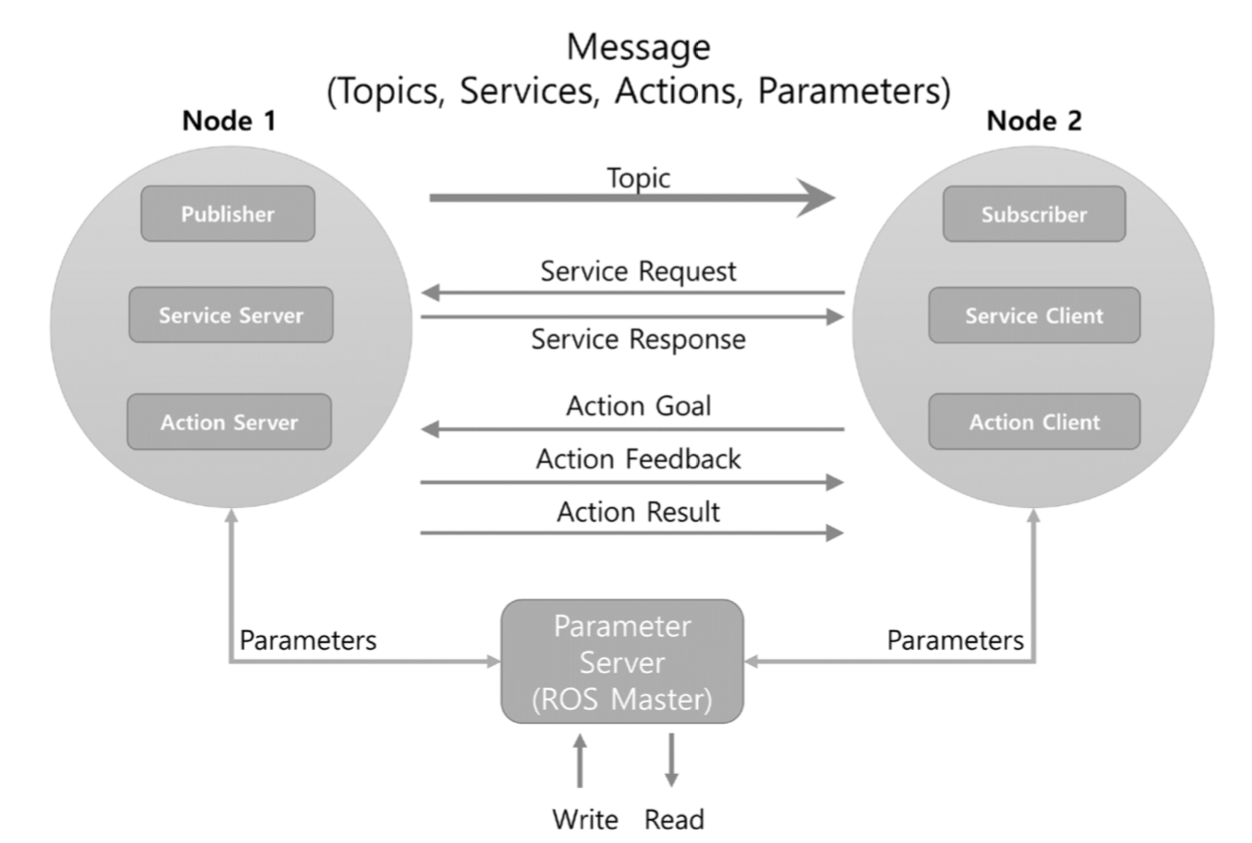
\includegraphics[width = 0.7\textwidth]{content/images/ch2/ros_message_communication.png}
    \caption{ROS Message Communication}
    \label{fig:ros_message_communication}
    \end{figure}
    
\subsection{ROS Tools}
ROS's core functionality is enhanced by a variety of tools and packages:

\begin{itemize}
    \item \textbf{Rviz.} Rviz\cite{RVIZ} is the 3D visualization tool of ROS. It can visualize information like the distance from a Laser Distance Sensor (LDS) to an obstacle, image value obtained from a camera, Point Cloud Data (PCD) of the 3D distance sensor such as RealSense, Kinect, or Xtion. As is shown in Figure \ref{fig:Rviz_gui}, multiple robot model and its path and laser data can be displayed.
    \begin{figure}[htbp]
        \centering
        \includegraphics[width = 0.7\textwidth]{content/images/ch2/Rviz_gui.png}
        \caption{Rviz Example: Navigation using TurtleBot 3 and Laser Distance Sensor (LDS)}
        \label{fig:Rviz_gui}
    \end{figure}

    \item \textbf{rqt.} rqt is an integration of more than 30 Qt-based ROS GUI development tool. It has plugins such as ``rqt\_tf\_tree'', ``rqt\_plot'' and  ``rqt\_graph''
   
    \item \textbf{rqt\_tf\_tree.} rqt\_tf\_tree is a type of rqt. It is a tool for visualizing the tree of frames being broadcast over ROS. Figure \ref{fig:tf_tree} presents the relative coordinate transformation (tf) of multi-robot system. If the poses of Laser Distance Sensor (LDS) are considered as the poses of the robots, the pose information of each robot is connected in the order of odom $\rightarrow$ base\_footprint $\rightarrow$ base\_link $\rightarrow$ base\_scan.
    
    \begin{figure}[htbp]
        \centering
        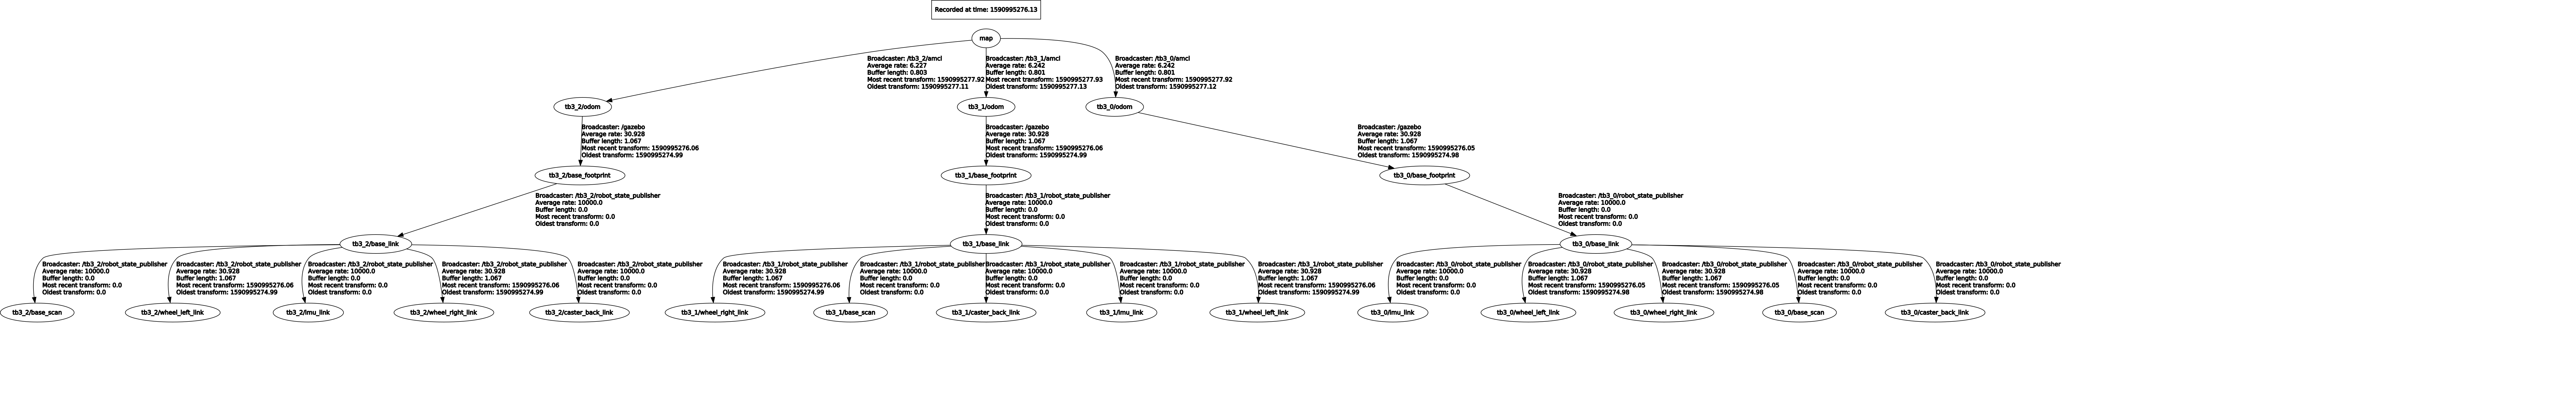
\includegraphics[width = 1.0\textwidth]{content/images/ch2/rqt_tree.png}
        \caption{rqt\_tf\_tree of Multi-robot Scheduling System}
        \label{fig:tf_tree}
        \end{figure}
       
    \item \textbf{rqt\_graph.} rqt\_graph is a type of rqt. It is a graphical tool that presents the status of nodes and topics. Figure \ref{fig:rqt_graph} presents relation of nodes in Multi-robot Scheduling System.
    \begin{figure}[htbp]
        \centering
        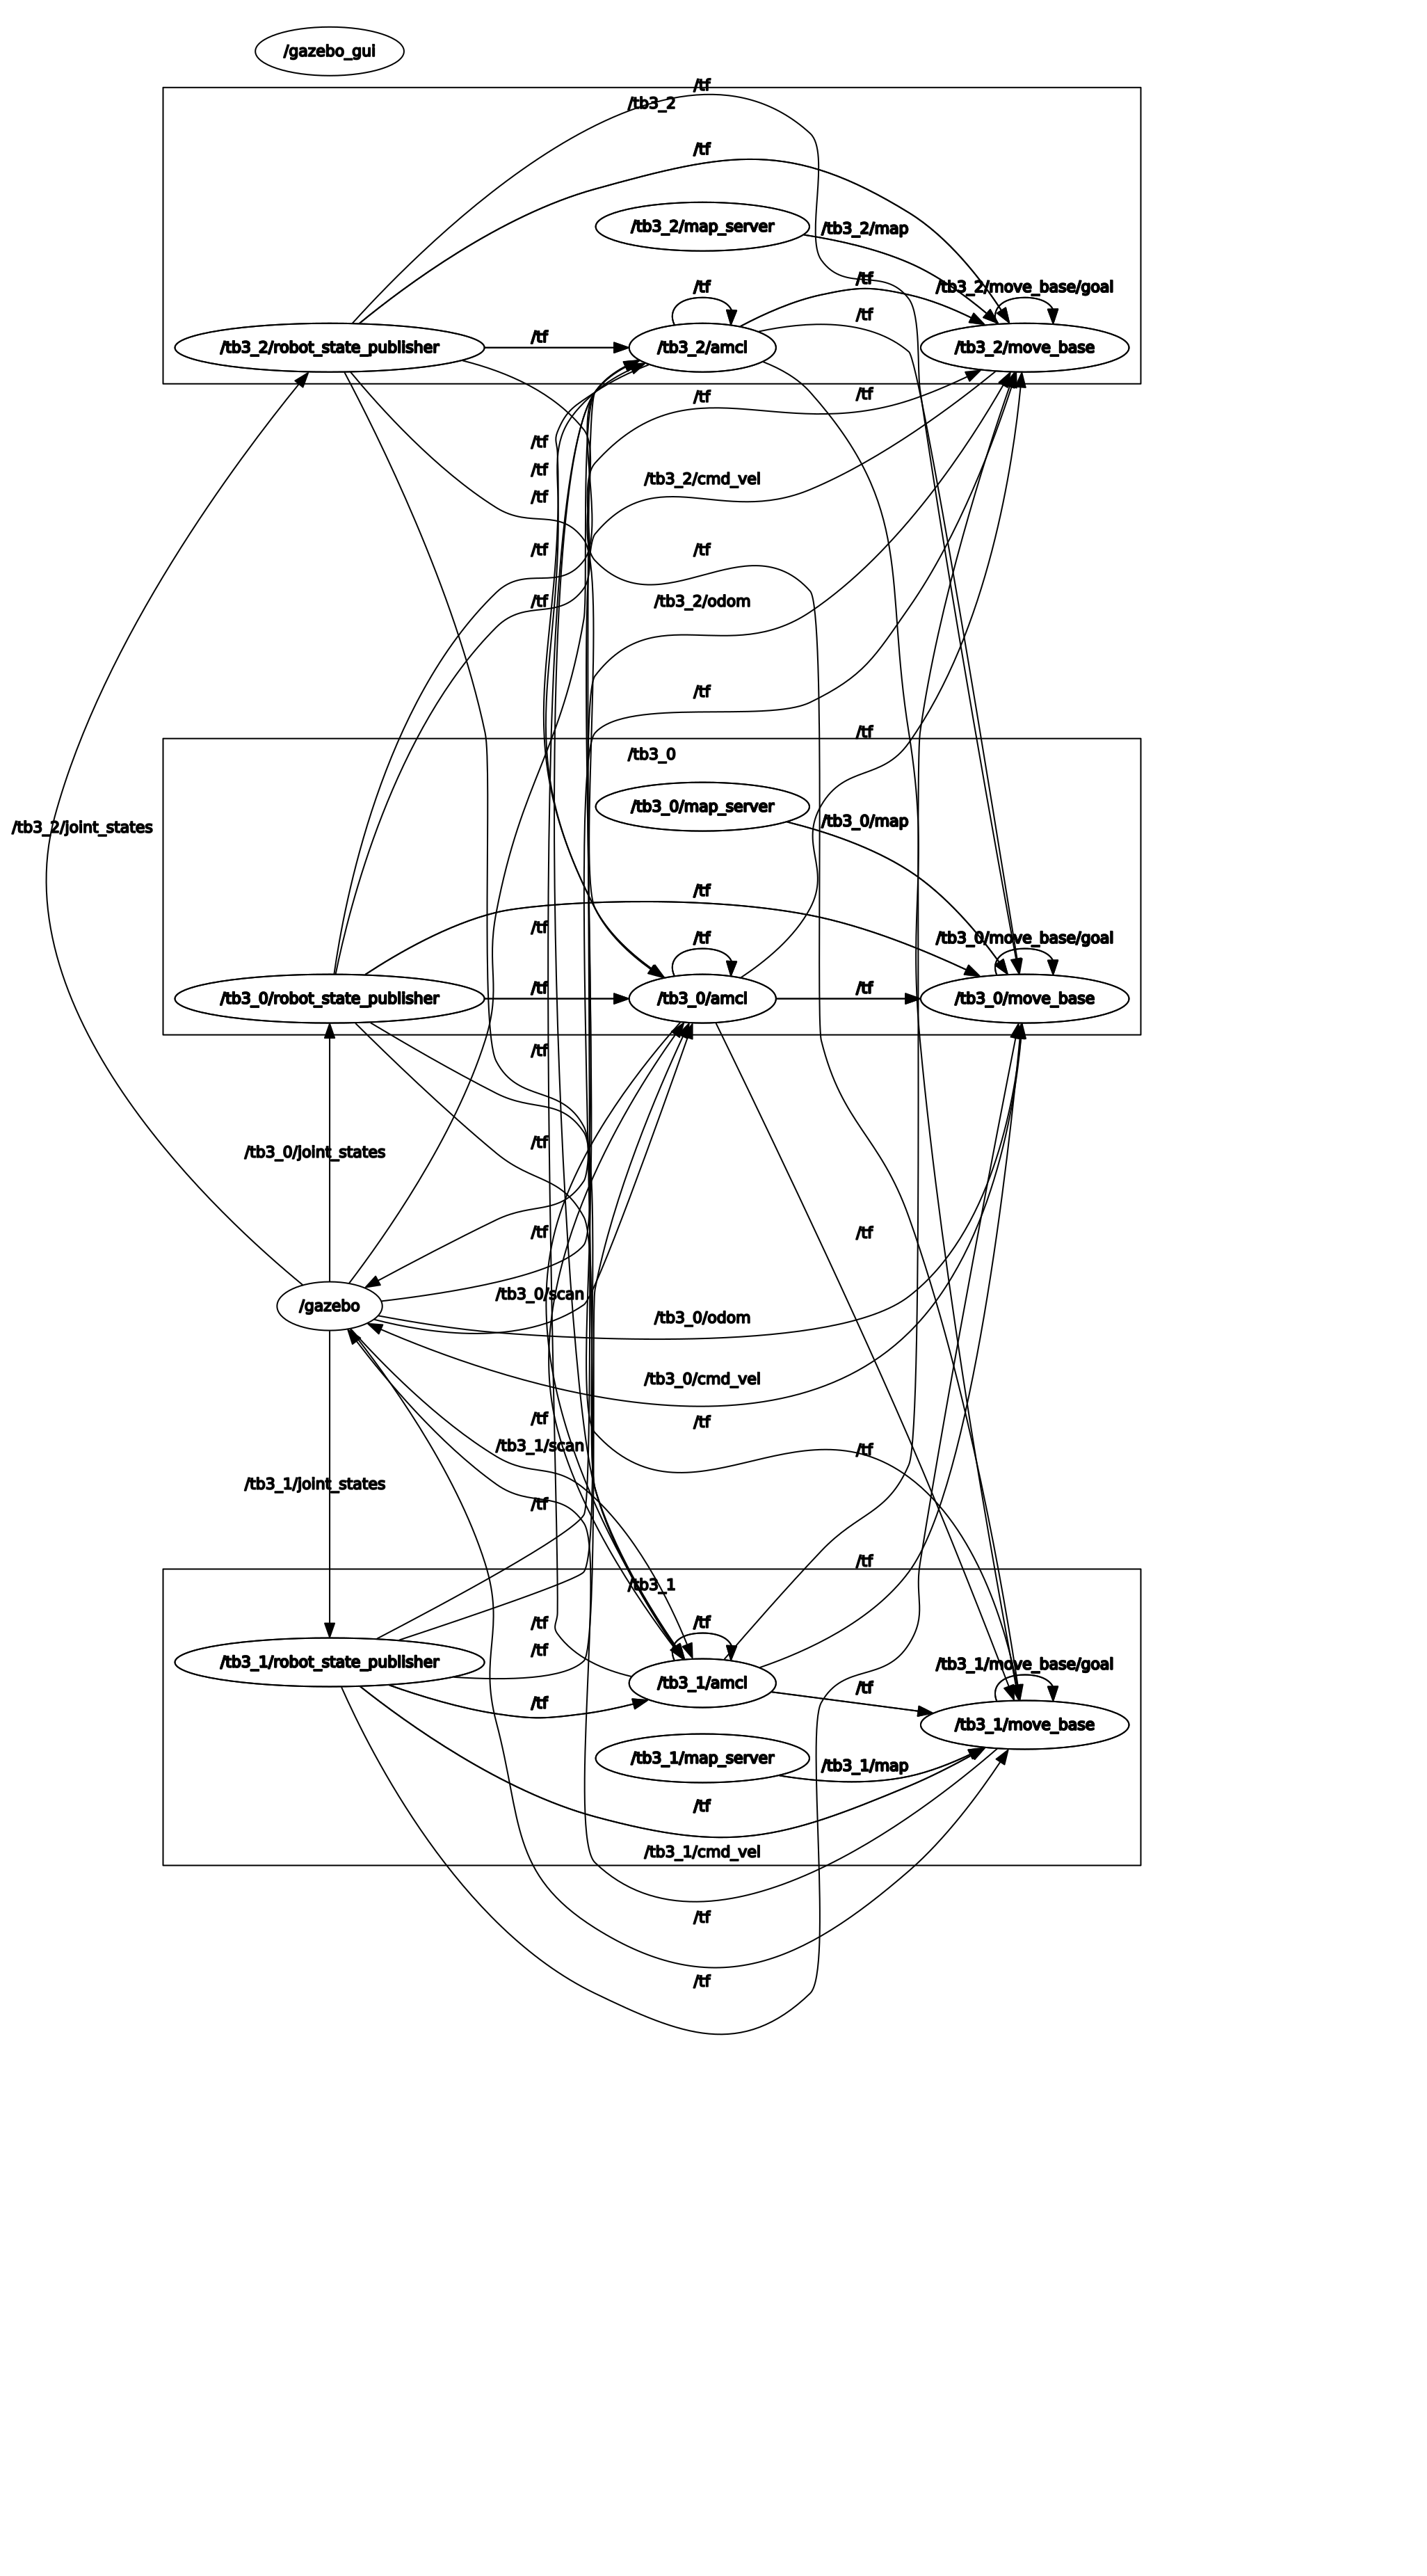
\includegraphics[width = 0.7\textwidth]{content/images/ch2/rosgraph.png}
        \caption{rqt\_graph of Multi-robot Scheduling System}
        \label{fig:rqt_graph}
    \end{figure}

    \item \textbf{Gazebo.} Gazebo \cite{GZ} is the 3D simulation tool integrated with ROS. The details of gezebo are introduced in Chapter \ref{sec:modeling_gazebo}.
\end{itemize}

\section{TurtleBot3 Simulation Using Gazebo}
\label{sec:modeling_gazebo}

\subsection{Gazebo Simulator}
Robot simulation is essential for robotics research, because it can pre-estimate the performance of robot algorithms before applying it to a real robot \cite{Afanasyev2015}. 
The simulator used in this project is Gazebo. Gazebo is a 3D dynamic indoor and outdoor multi-robot simulator integrated with ROS, and it offers physics simulation at a much higher degree of fidelity, a suite of sensors, and interfaces for both users and programs \cite{GZ}. 
Using Gazebo simulator affords to create new 3D model with geometrical primitive or import existing simulated robots and environments. 

\subsection{TurtleBot3 Robot}
The robot model used in this project is TurtleBot3 Burger. Because it is a small, affordable, programmable ROS-based mobile robot for use in research and prototyping. 
As is shown in Figure \ref{fig:robot_hardware}, the basic components are actuators, an SBC (Single-Board Computer) for operating ROS, a LDS sensor for SLAM (Chapter \ref{sec:navigation}) and navigation, restructurable mechanism, an OpenCR embedded board used as a sub-controller, sprocket wheels that can be used with tire and caterpillar, and a 3 cell lithium-poly battery.
The simulated robot (Figure  \ref{fig:simulated_robot}) has a similar outfit. In addition, Gazebo simulates the robot locomotion and sensor measurements used for localization and navigation, and exports the simulation results to ROS.


\begin{figure}[htbp]
\centering
\begin{minipage}[t]{0.48\textwidth}
\centering
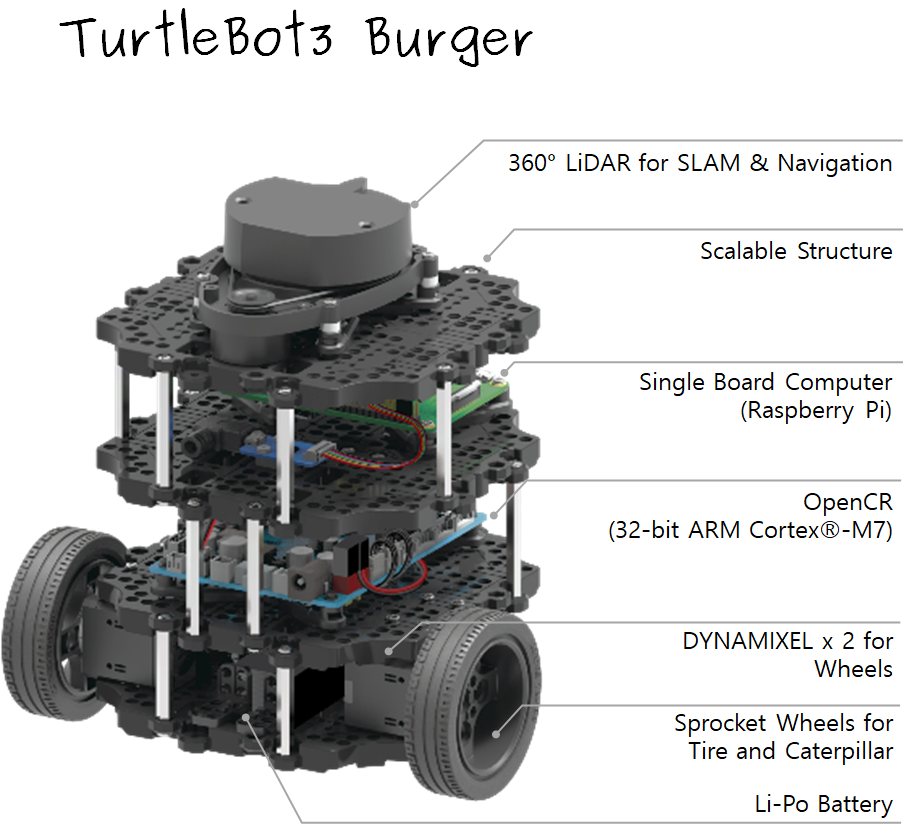
\includegraphics[width=6cm]{content/images/ch2/turtlebot3_burger_components.png}
\caption{Robot Hardware Configuration}
\label{fig:robot_hardware}
\end{minipage}
\begin{minipage}[t]{0.48\textwidth}
\centering
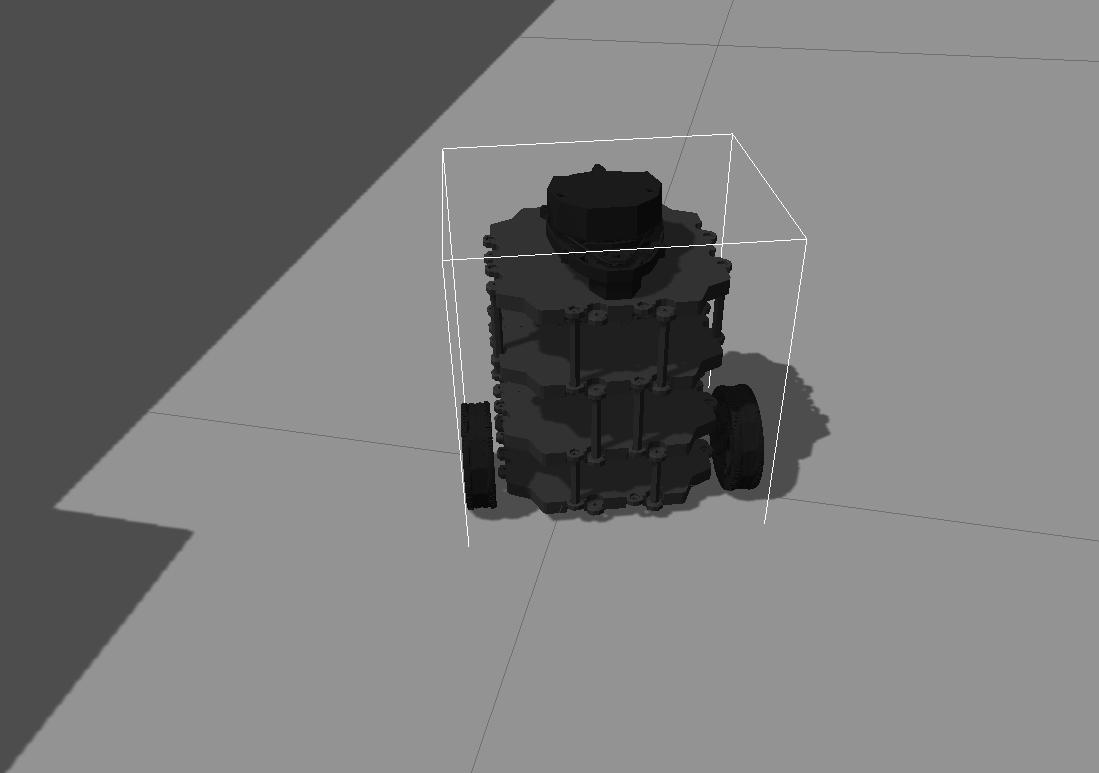
\includegraphics[width=6cm]{content/images/ch2/robot_model.jpg}
\caption{Robot 3D Modeling in Gazebo}
\label{fig:simulated_robot}
\end{minipage}
\end{figure}

\subsection{3D Modeling of Indoor Environment}

In this project we selected a model exactly the same as the floor of the department as a trial 3D model (Figure \ref{fig:modeling_environment_gazebo}).
This model is a typical office environment that contains a corridor along the central x-axis and 16 rooms located around the corridor. 

\begin{figure}[htbp]
    \centering
    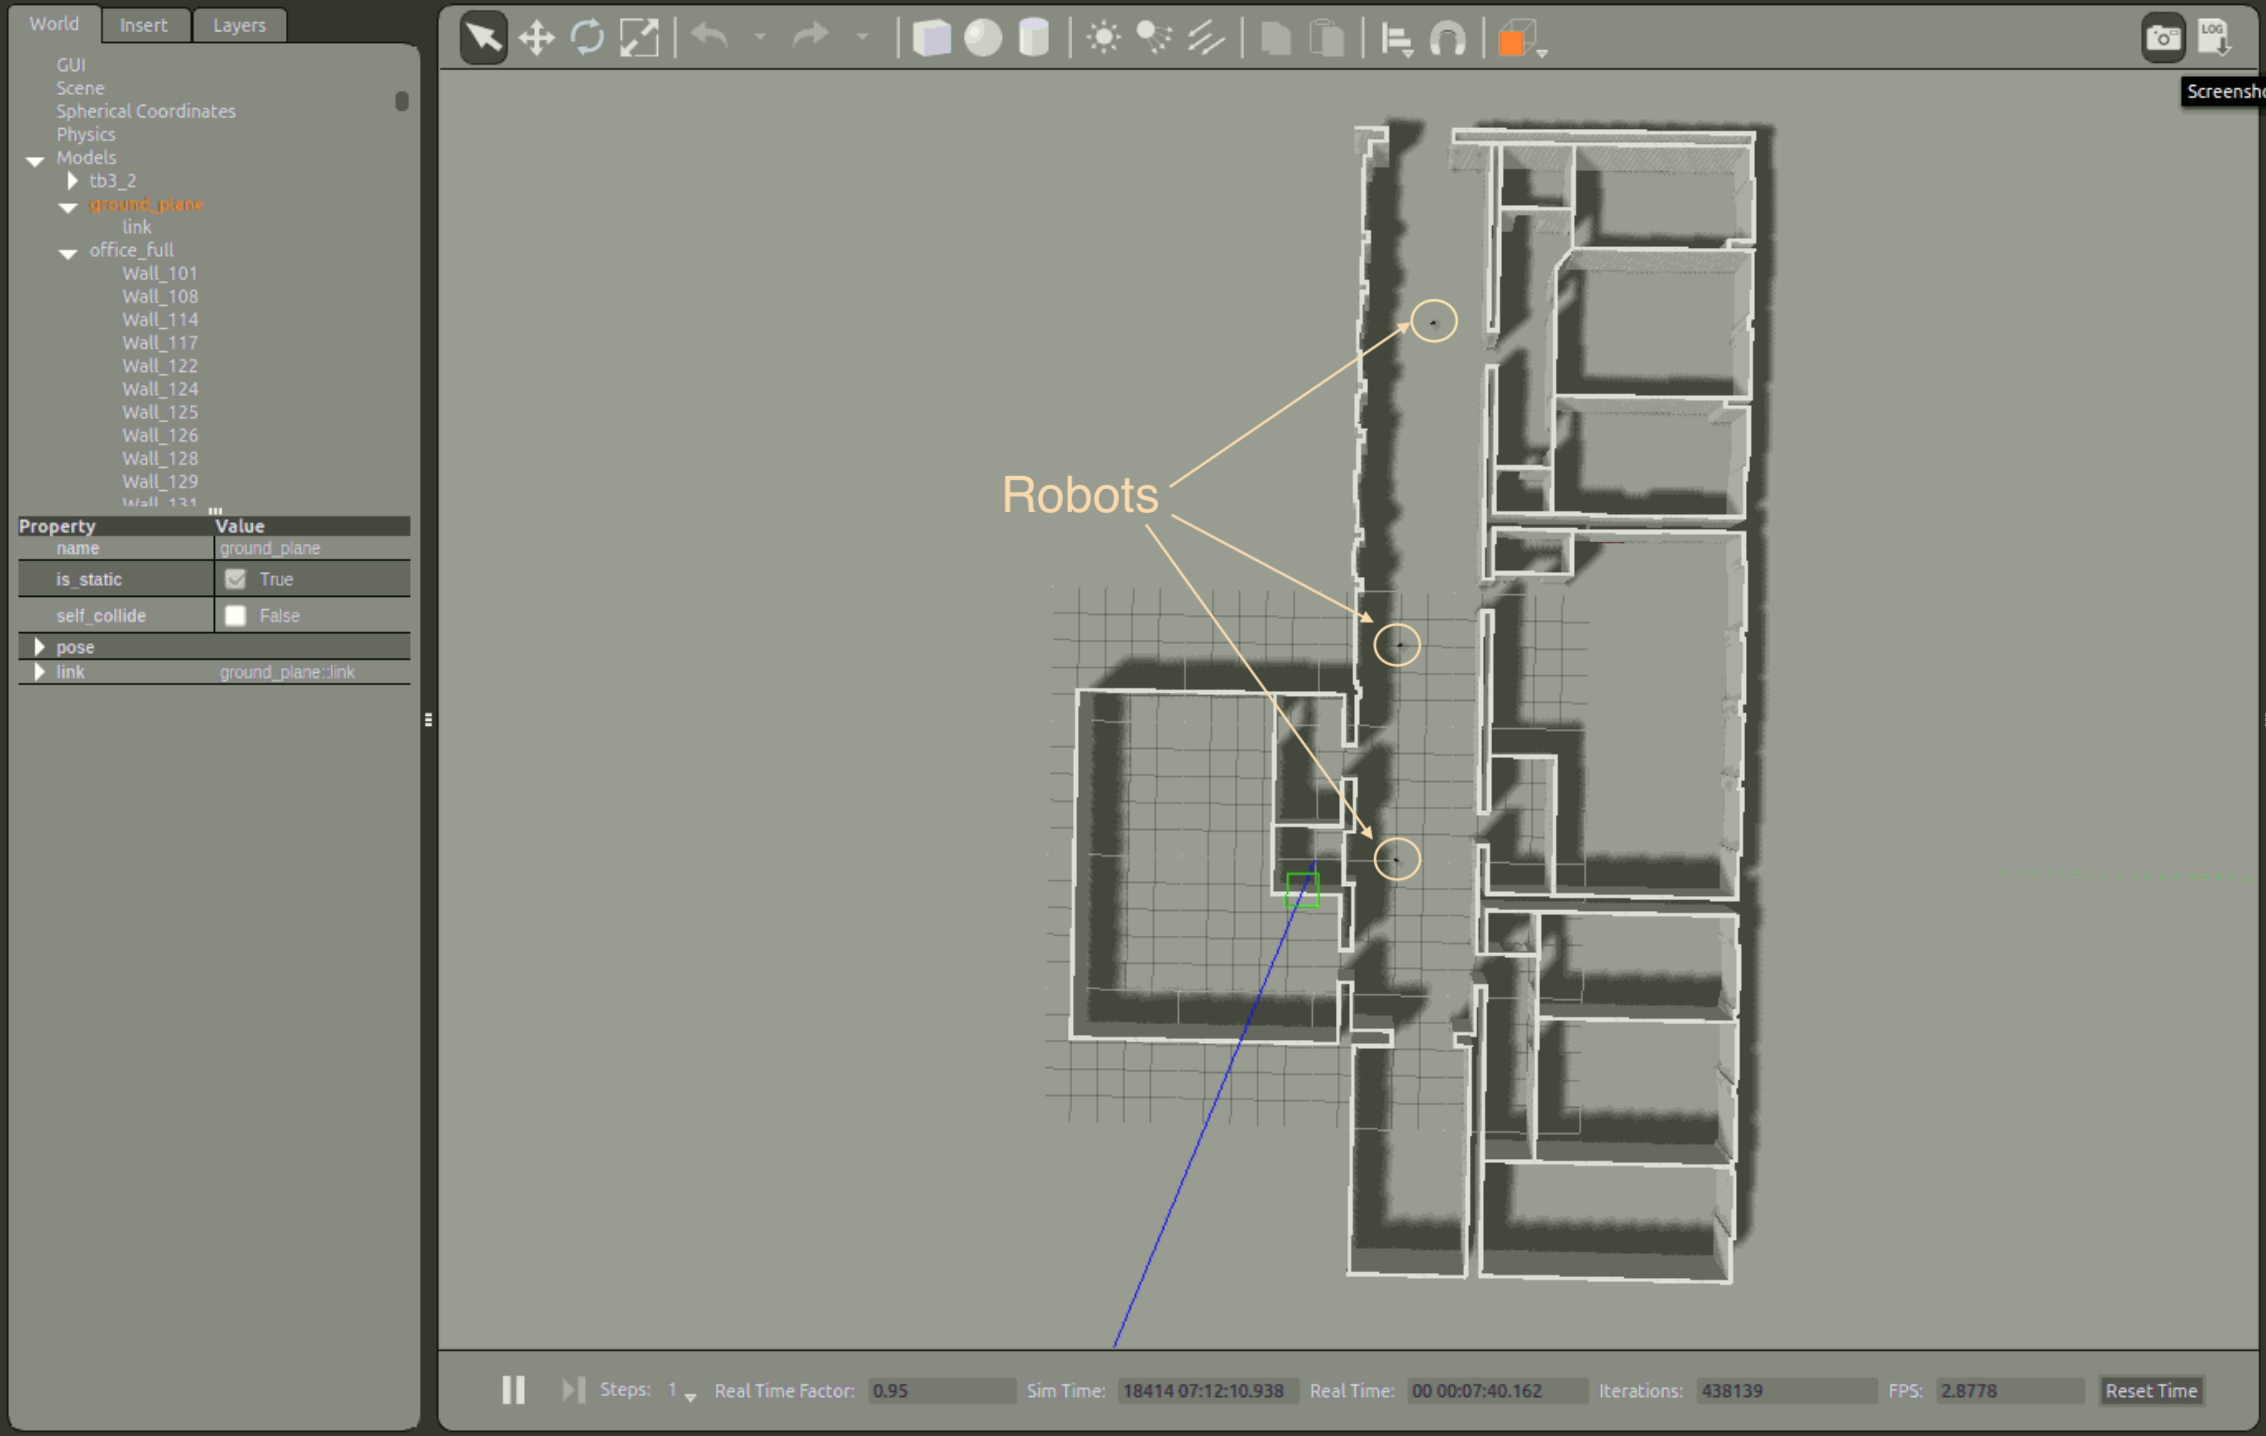
\includegraphics[width = 0.7\textwidth]{content/images/ch2/gazebo_gui_environment.png}
    \caption{3D Modeling of Indoor Environment in Gazebo}
    \label{fig:modeling_environment_gazebo}
\end{figure}

\section{Robot Navigation and Virtual SLAM}
\label{sec:navigation}

There are essential technologies to realize autonomous robot navigation: 
\begin{enumerate}
    \item \textbf{Having map of the given environment.} In this project, SLAM(Simultaneous Localization Ana Mapping) is used to create a map of the given environment. Using SLAM, the robot explores the unknown spaces and detects its surrounding areas and estimates its current location as well as creating a map. The steps of executing virtual SLAM with TurtleBot3 is shown in Website \cite{T3SLAM}. Once the robot finish exploring the indoor environment, an occupancy grid map (OCM) is generated (Figure \ref{fig:occupancy_grid}).
    \item \textbf{Measuring or estimating the pose of robot.} Pose is consists of position and orientation. The dead reckoning \cite{DEADRECKONING} is the most popular indoor pose estimation method for the robot. The amount of movement of robot is measured with the rotation of the wheel. However, the error between the calculated distance with wheel rotation and the actual travel distance increases over time. Therefore, the inertial measurement unit (IMU) sensor\cite{Woojin17} is used to measure triaxis angular velocities and triaxis acceleration to estimate the position of the mobile robot.  This inertial data can be used to compensate the error of position and orientation between calculated value and the actual value.
    \item \textbf{Avoiding obstacles such as walls and furniture.} The laser-based distance sensor on robot are widely used in figuring out whether there are obstacles including walls, furniture and other robots. The common laser-based distance sensor includes LDS (Laser Distance Sensor), LDF (Laser Doppler flowmetry) and LiDAR (Light Detection And Ranging) and ultrasonic sensors and infrared distance sensors. The TurtleBot3 equips 360 Laser Distance Sensor LDS-01. The visualization of Laser data in Rviz is shown in Figure \ref{fig:Rviz_gui}.
    \item \textbf{Finding the optimal route calculation and driving.} It is important to find the optimized route to the destination. There are many algorithms that perform path searching and planning such as A* algorithm\cite{ASEARCH}, potential field\cite{POTENTIAL}, particle filte\cite{PARTICLE}, and RRT (Rapidly-exploring Random Tree)\cite{RRT}.
    \begin{figure}[htbp]
        \centering
        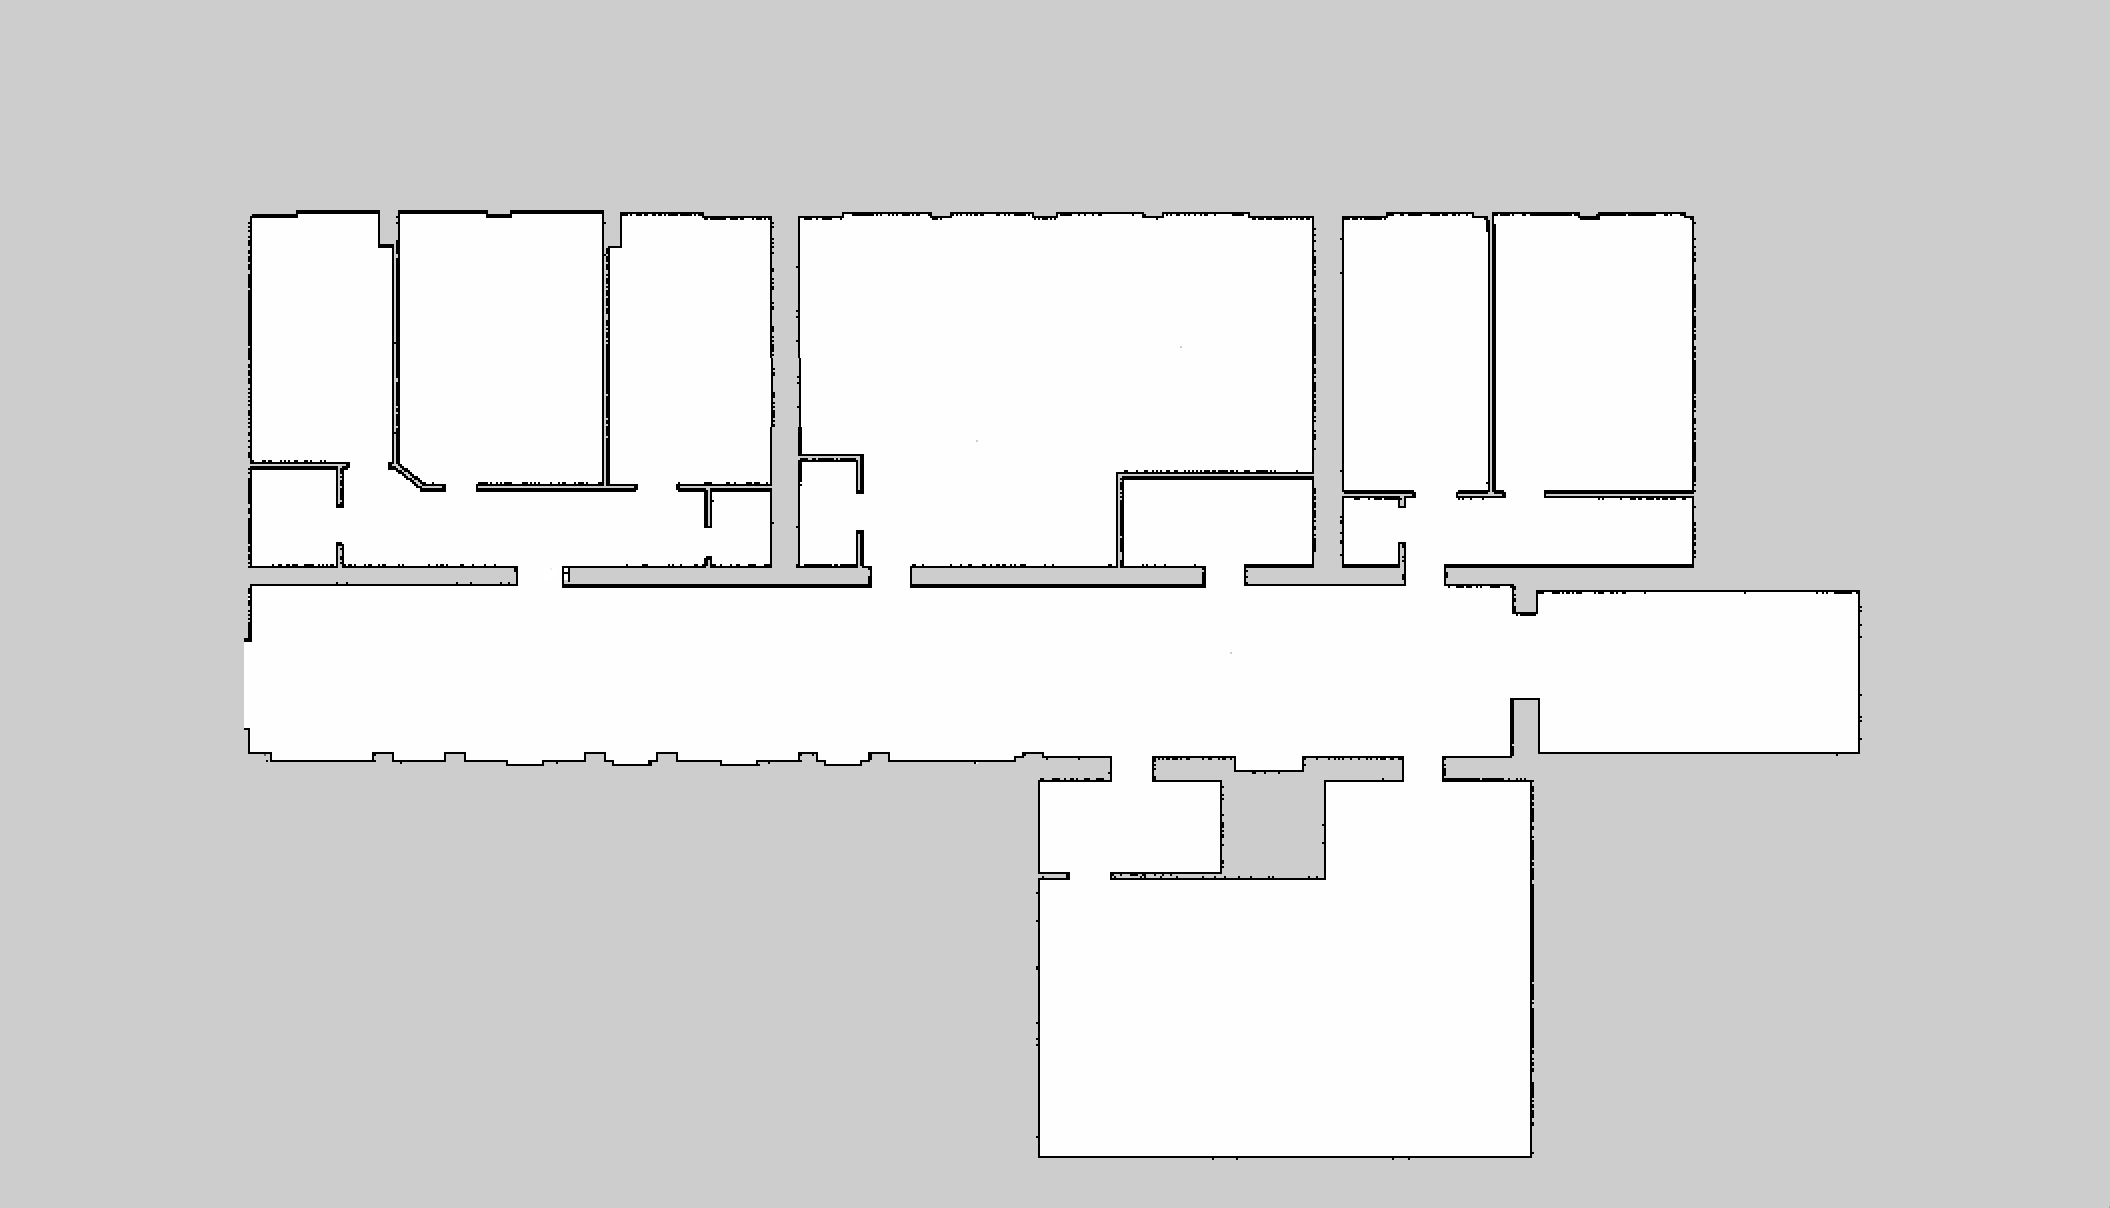
\includegraphics[width = 0.7\textwidth]{content/images/ch2/occupancy_grid.png}
        \caption{Occupancy Grid Map (OGM). White presents the free area in which robots can move, black presents the occupied area in which robots can not move, and gray is the unknown area.}
        \label{fig:occupancy_grid}
    \end{figure}
\end{enumerate}


\section{Exist Task Scheduling Methods}
\label{sec:exist_task_scheduling_methods}
So far, the background information such as tools and important concepts of ROS are introduced. This Chapter discusses some popular methods of task scheduling. Those task scheduling methods can be divided into centralized methods and distributed methods.

\subsection{Centralized Method vs. Distributed Method}
In the case of centralized method, a centralized schedule collects all task requests and uses resource utilization information to schedule tasks. The centralized method is easy to manager and faster to repair in case of failure. However, the autonomy of the robots in pure centralized method is limited becaued all robots only execute commands from centralized scheduler and not determine what tasks to do \cite{NUNES201755}. In addition, since the centralized scheduler must compute all resources and tasks, the centralized system is difficult to scale to large-size network \cite{CHRISTODOULOPOULOS20091172}.
Chapter \ref{sec:constraint_programming} introduces a centralized constraint programming method. Chapter \label{sec:genetic_method} introduces a centralized method based on A* and Genetic Algorithm.

In the case of distributed method, there are multiple distributed schedulers keep tracking the resource availability and use this information to perform task scheduling\cite{CHRISTODOULOPOULOS20091172}. This method distributes the associated computation overhead, as a result it eliminates the bottleneck caused by the centralized scheduler and improves the scalability and realiability and scalability if the network. The challenge in distribute method is the coordination of distribute schedulers as well as the required control plane overhead \cite{CHRISTODOULOPOULOS20091172}.
Chapter \ref{sec:auction_method} introduces a distributed auction method. Chapter \ref{sec:global_unit_method} introduces a communication-efficient distributed method. 

\subsection{Centralized Constraint Programming Method}
\label{sec:constraint_programming}
Booth has proposed a multi-robot system that support elderly residents in a retirement home setting in  \cite{retire2017}. The robots search for elderly residents in the environment in the morning, eliciting their availability and preferences for activities. The centralized scheduler then use constraint programming method to allocate these assistive activities over the day. Those problem-specific constrains includes robot energy consumption, activity priority, robot-user activity synchronization, user location, and user availability carlendar that identifies their busy intervals. Once this information is attained, the system allocate and schedule activities to robots for the day before executing the plan.

\subsection{Centralized Method based on A* and Genetic Algorithm}
\label{sec:genetic_method}
Chun has proposed a centralized task scheduling and path-planning method based on A* and Genetic Algorithm \cite{Chun12}.
In this research work, Genetic Algorithm is responsible for task scheduling to find the optimal solution for industrial plant inspection problems, and A* Algorithm is used to calculate the traveling cost and path-planning of a robot moving from one position to another, because it can consider more detail path conditions such as obstacles, furnitures and different terrain conditions. The traveling cost is one evaluation parameter of the fitness function in the GA, but in this research it is referred to the completion time. To be more precise, it is the time period of the first robot starting its tasks and the last robot finishing its tasks.
The goal of the task scheduling method is to find an ordered set of tasks for robots in order to minimize the completion time while decreasing the total power consumption.
Two Greedy algorithms are proposed for task assignment. The first one is to find one task for each robot which provides for the minimum completion time in each step in order to minimize the total completion time. The second one is to find only one robot-task pair which takes the minimum time in each step in order to decrease the total power consumption. 

\subsection{Distributed Auction Method}
\label{sec:auction_method}
When system performs a long-term task allocation process, the communication link between costumer agent and robots may be disconnected. This may cause a conflict or failed assignment. 
Distributed methods are more suitable in this case as distribute the computation to individual agents \cite{NUNES201755}. 
Dong-Hyun Lee has proposed a resource-oriented, distributed auction algorithm \cite{Dong2015}. The customer agents and robots with limited communication ranges construct an ad-hoc network tree. The customer agent becomes auctioneer and broadcasts an auction call to the task. The robots become bidders and submit their bid values to the customer agent. The bid values consider local information such as the tasks in robot task queue, robot's resource levels and estimated travel distance and time for multiple path. Since each path consists of different charging stations, the robot's resource levels after completing a task and estimated travel time depends on the path. After receiving all bid values, the agent assigns the task to the robot with the lowest bid value. This senarios not only avoids unexpected battery drain while robot processing task, but also let robots maintain high capacities. 

\subsection{Distributed Method with Global Unit}
\label{sec:global_unit_method}
Kashyap Shah proposed a communication-efficient distributed dynamic task scheduling system with a shared global unit \cite{Shah7}. Each robot can make its own decision through communicating with other robots as well as check and update the current task status in the global unit. Besides, this method considers two dynamic environment. 
Firstly, some robots maybe no long be able to handle its current task because the task environment has changed. In this case the defective robot check the global unit and send a help message to robots which can handle the task. Secondly, some robot may fail under the dynamic environment. This robot failure will be detected by tracking the communication signal and its status in the global unit will be updated as failed to make sure no more tasks will be allocated to this robot. In addition, if the failed robot is running a task, its current task will be reassigned to another robot. 

\section{Exist Quantities of Cost Function}
\label{sec:cost_function}
One of the most important steps when designing a multi-robot task scheduling algorithm is calculating the costs of tasks. Jia summaries several physical quantities used in algorithm's cost in \cite{Jia2013ASA}. In their study it can be concluded that the most common used decision variables are estimated travel distance and time, as proposed in \cite{Dong2015}. Other kinds of decision variables involved are the number of traversals and energy consumed. 
In addition, Korsah proposed a comprehensive taxonomy of multi-robot task scheduling problems that explicitly takes into consideration the issues of interrelated utilities and constraints. In this taxonomy, tasks are distinguished by decomposability and multi-agent-allocatability \cite{Korsah13}.
In the case of Chun's method \cite{Chun12}, the cost is defined as completion time. There are a group of m robots $R = {R1,R2,...,Ri,...,Rm}$, a set of n tasks $T = {T1,T2,...,Tj,...,Tn}$ with relative weights ${w1, w2, ..., wj , ...wn}$. The cost $Cij$ of robot $Ri$ executing task $Tj$ is defined as the completion time which is the time span of the first robot starting its tasks and the last robot finishing its tasks.
The cost function J is:

\begin{equation}
	\label{eq:large_execute_task_cost} 
	\begin{aligned}
    & J = max( \sum_{j=1}^n C_{1j}, \sum_{j=1}^n C_{1j},\dot,\sum_{j=1}^n C_{ij},\dot,\sum_{j=1}^n C_{mj})\\
    &  C_{ij} = \left\{
            \begin{array}{lr}
            > 0, & \mbox{if robot Ri is allocated task Tj := 0}\\
            :=0 &  \mbox{otherwise}
             \end{array}
        \right.
	\end{aligned}
\end{equation}
 %Materials and Methods
\chapter{Approach}
% Describe the performed solution with all possible details. Define necessary parameters, inputs, outputs and context of use, possible problems and when they can be applied. 

% Remember to define necessary concepts before using them, building the text from easiest definitions (not depending on previous definitions) to complex definitions (depending on previous definitions).

% E.g: 
% \begin{itemize}
%	\item Lost Communication: a lost communication occurs when the conditions of the environment are not sufficient or the distance between sender and receiver is to hight to transmit information.
%	\item Wait until rescue: when the robot loses its communication, the pre-designed state machine will stop the motors to keep the actual position. Energy safe mode will be enabled, at the same time that a channel transceiver daemon will send SOS messages every T and wait for reply during T sec. 
%\end{itemize}
In our system there are multiple robots that must handle various tasks. For example, visiting given rooms. To tackle this problem, a communication efficient task allocation system is designed. 
This system allocate task according to system resources, including environment factors, robot status and task specifications. Once this information is attained, the task allocation system assign robot a set of task.

\begin{itemize}
	\item \textsl{Robot.} Each robot is responsible for moving in 2-dimensional physical space as well as gathering measurement result from sensors. It has a rechargeable battery, and its level drops as robot moves and rotates.
	\item \textsl{Tasks.} Each task requires one or more robots to traverse a path in the workspace and carry out certain actions\cite{Ivan2017}.
	\item \textsl{Environment.} In this project, all robots are considered moving in an office environment that contains a corridor along the central x-axis and 16 rooms located around the corridor. The environment factors, such as room locations and occupancy possibilities help task allocation.
\end{itemize}

\section{Architecture Design}

The architecture of the system consist of several parts: centralized pool, robot controller, navigation stack, charging station and system environment(Figure \ref{fig:system_architecture}). 
\begin{itemize}
	\item \textsl{Centralized Pool.} A centralized pool consist of several modules: multi-robot task allocation module, map information, database, execution and monitoring. The database and map information modules contain the environment information(Figure \ref{fig:database_er}). The execution and monitoring module interacts with robots. The multi-robot task allocation module allocate tasks to robots.
	\item \textsl{Robot Controller.} A robot controller contains several modules: local task queue, execution and robot action. The local task queue stores tasks that the robot needs to complete sequentially. The execution module receives commands from centralized pool and decides when and which task the robot should run. The robot action module run tasks in local task queue when receives decision from execute module and interacts with enviroment and its navigation stack.
	\item \textsl{Navigation stack.} The move\_base node provides a ROS interface for configuring, running, and interacting with the navigation stack on a robot. It makes robot move to desired positions using the navigation stack. Its advantages include optionally performing recovery behaviors when the robot perceives itself as stuck\cite{move_base_node}. 
\end{itemize} 

\begin{figure}[htbp]
	\centering
	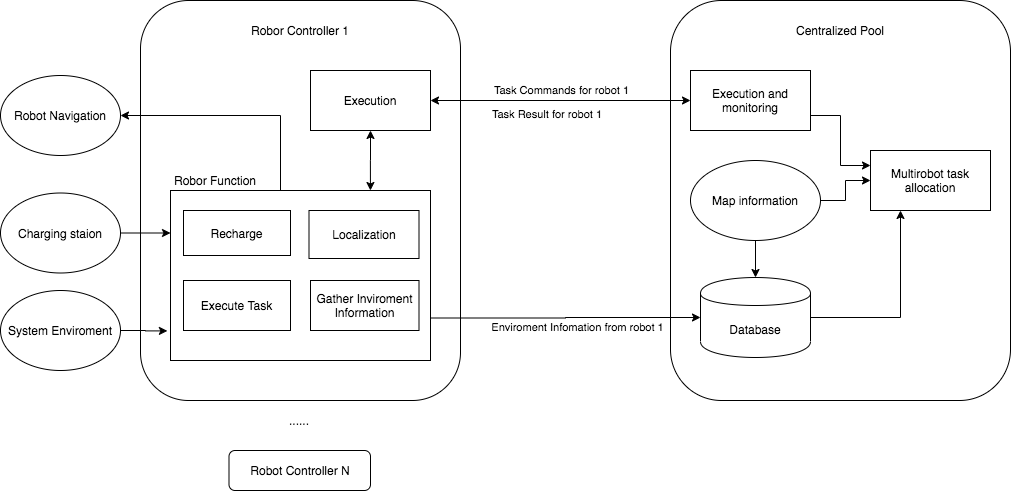
\includegraphics[width = 0.9\textwidth]{content/images/ch3/architecture.drawio.png}
	\caption{System Architecture}
	\label{fig:system_architecture}
\end{figure}

\section{Environment and Gather Environment Infomation Approach}
\subsection{System enviroment}
\label{sec:system_enviroment}
As is discussed in the previous section, the system environment is an office environment. The SLAM (Simultaneous Localization and Mapping) is a technique to draw a map by estimating current location in an arbitrary space \cite{slam}. Map (Figure \ref{fig:room_division}) is created by SLAM.

\paragraph{Important areas and coordinates:}
\begin{itemize}
	\item \textsl{Rooms.} The enviroment is divided into regions that represent rooms in the facility (Figure \ref{fig:room_division}). If the coordinates of a point are in a region, it can be judged that the point is located in the corresponding room.
	\item \textsl{Doors.} The positions of doors (Figure \ref{fig:positions_door_station}) are stored in database. There are used by a ROS door simulator node, which broadcasts positions and door status periodically. The broadcast messages are received and filtered by robots.
	\item \textsl{Charging Stations.} The positions of charging stations (Figure \ref{fig:positions_door_station}) are used by ROS charging station nodes. For details please refer to Section \ref{sec:charging_station}.
\end{itemize}

\begin{figure}[htbp]
	\centering
	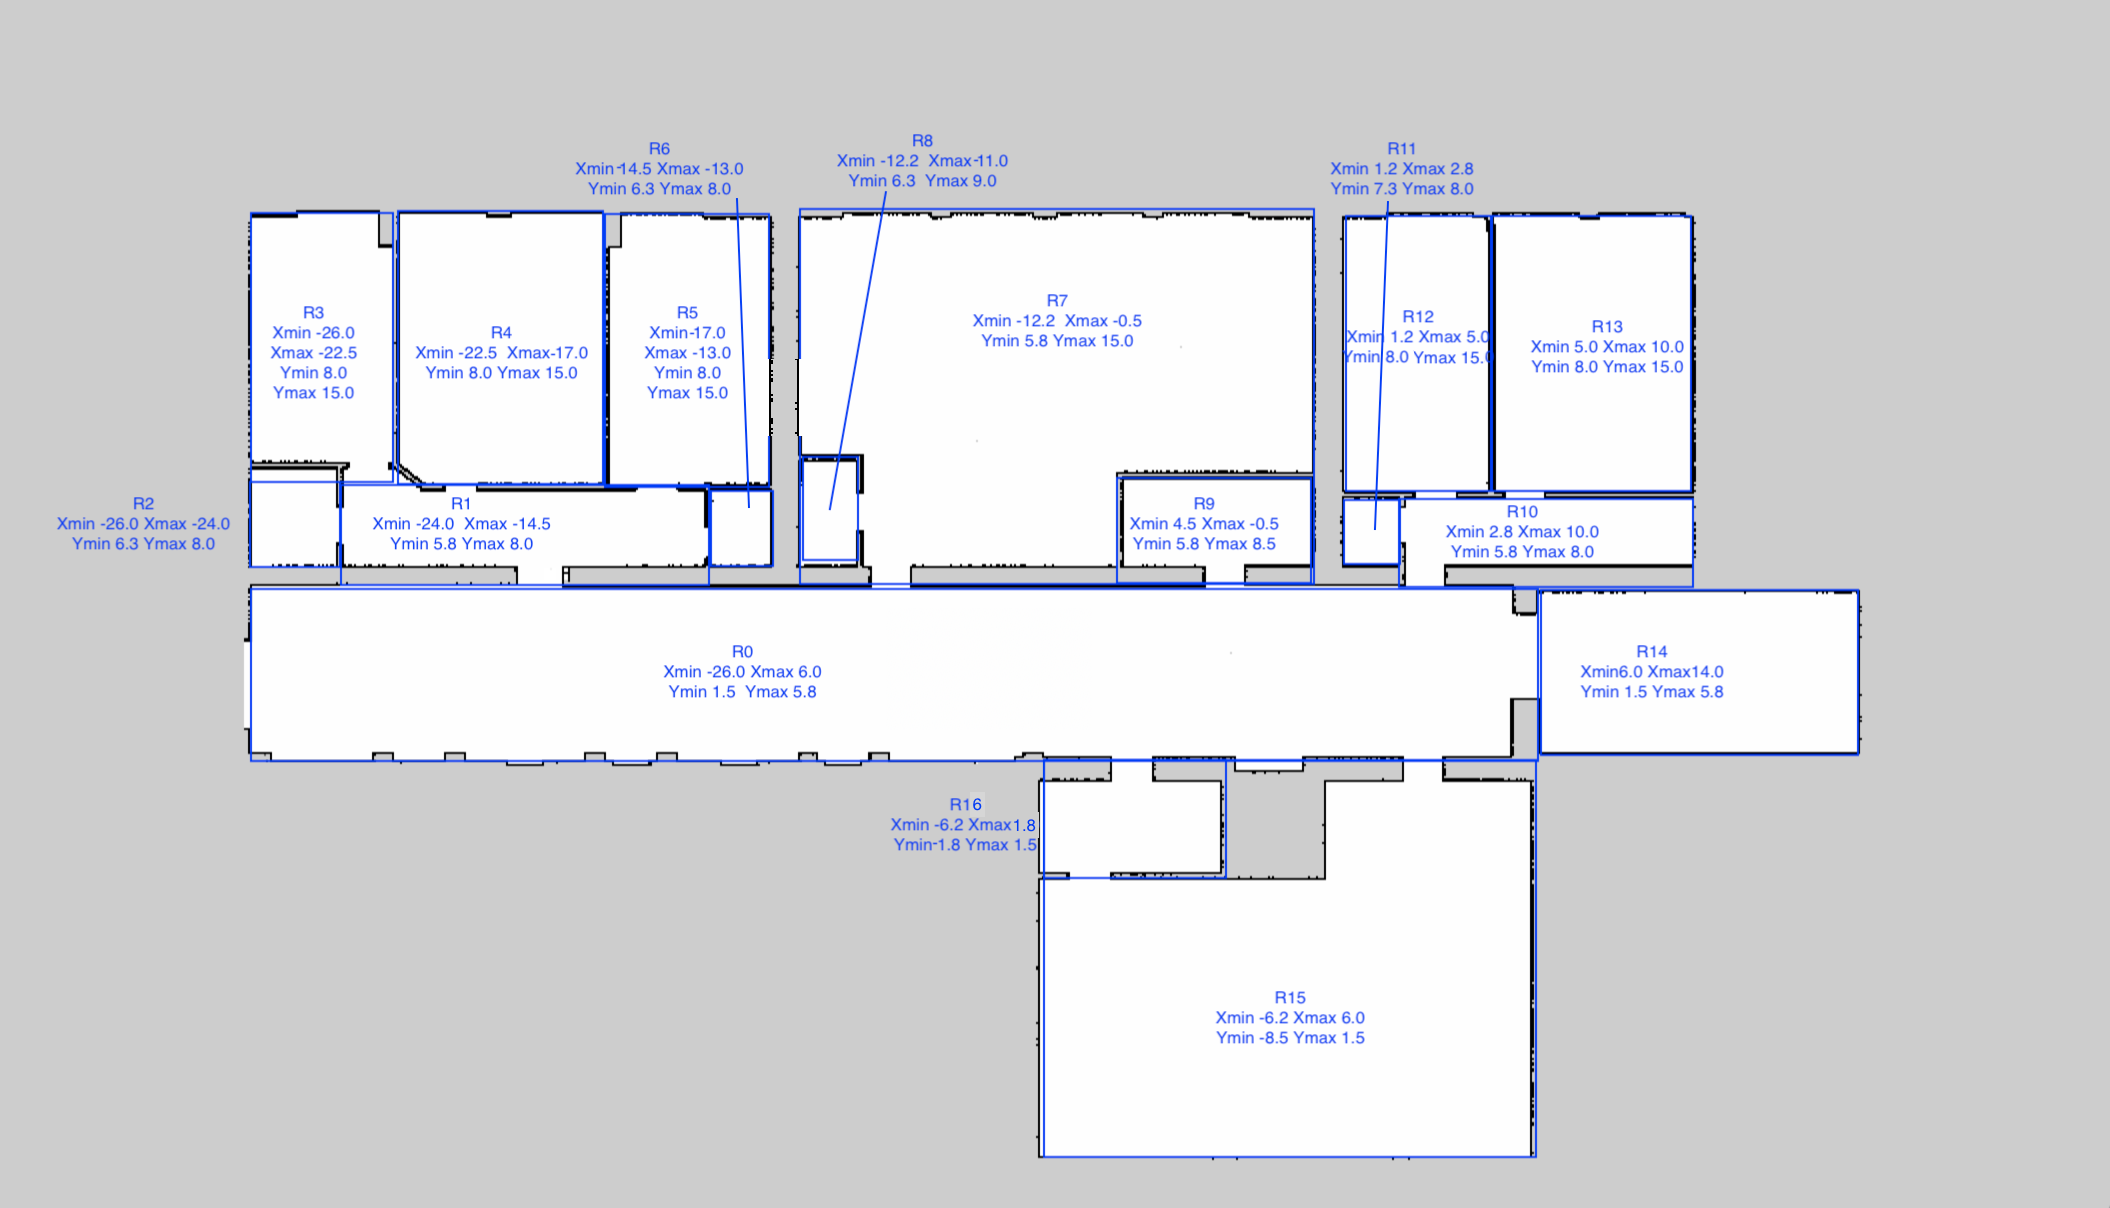
\includegraphics[width = 0.9\textwidth]{content/images/ch3/room_division.png}
	\caption{Room division}
	\label{fig:room_division}
\end{figure}

\begin{figure}[htbp]
	\centering
	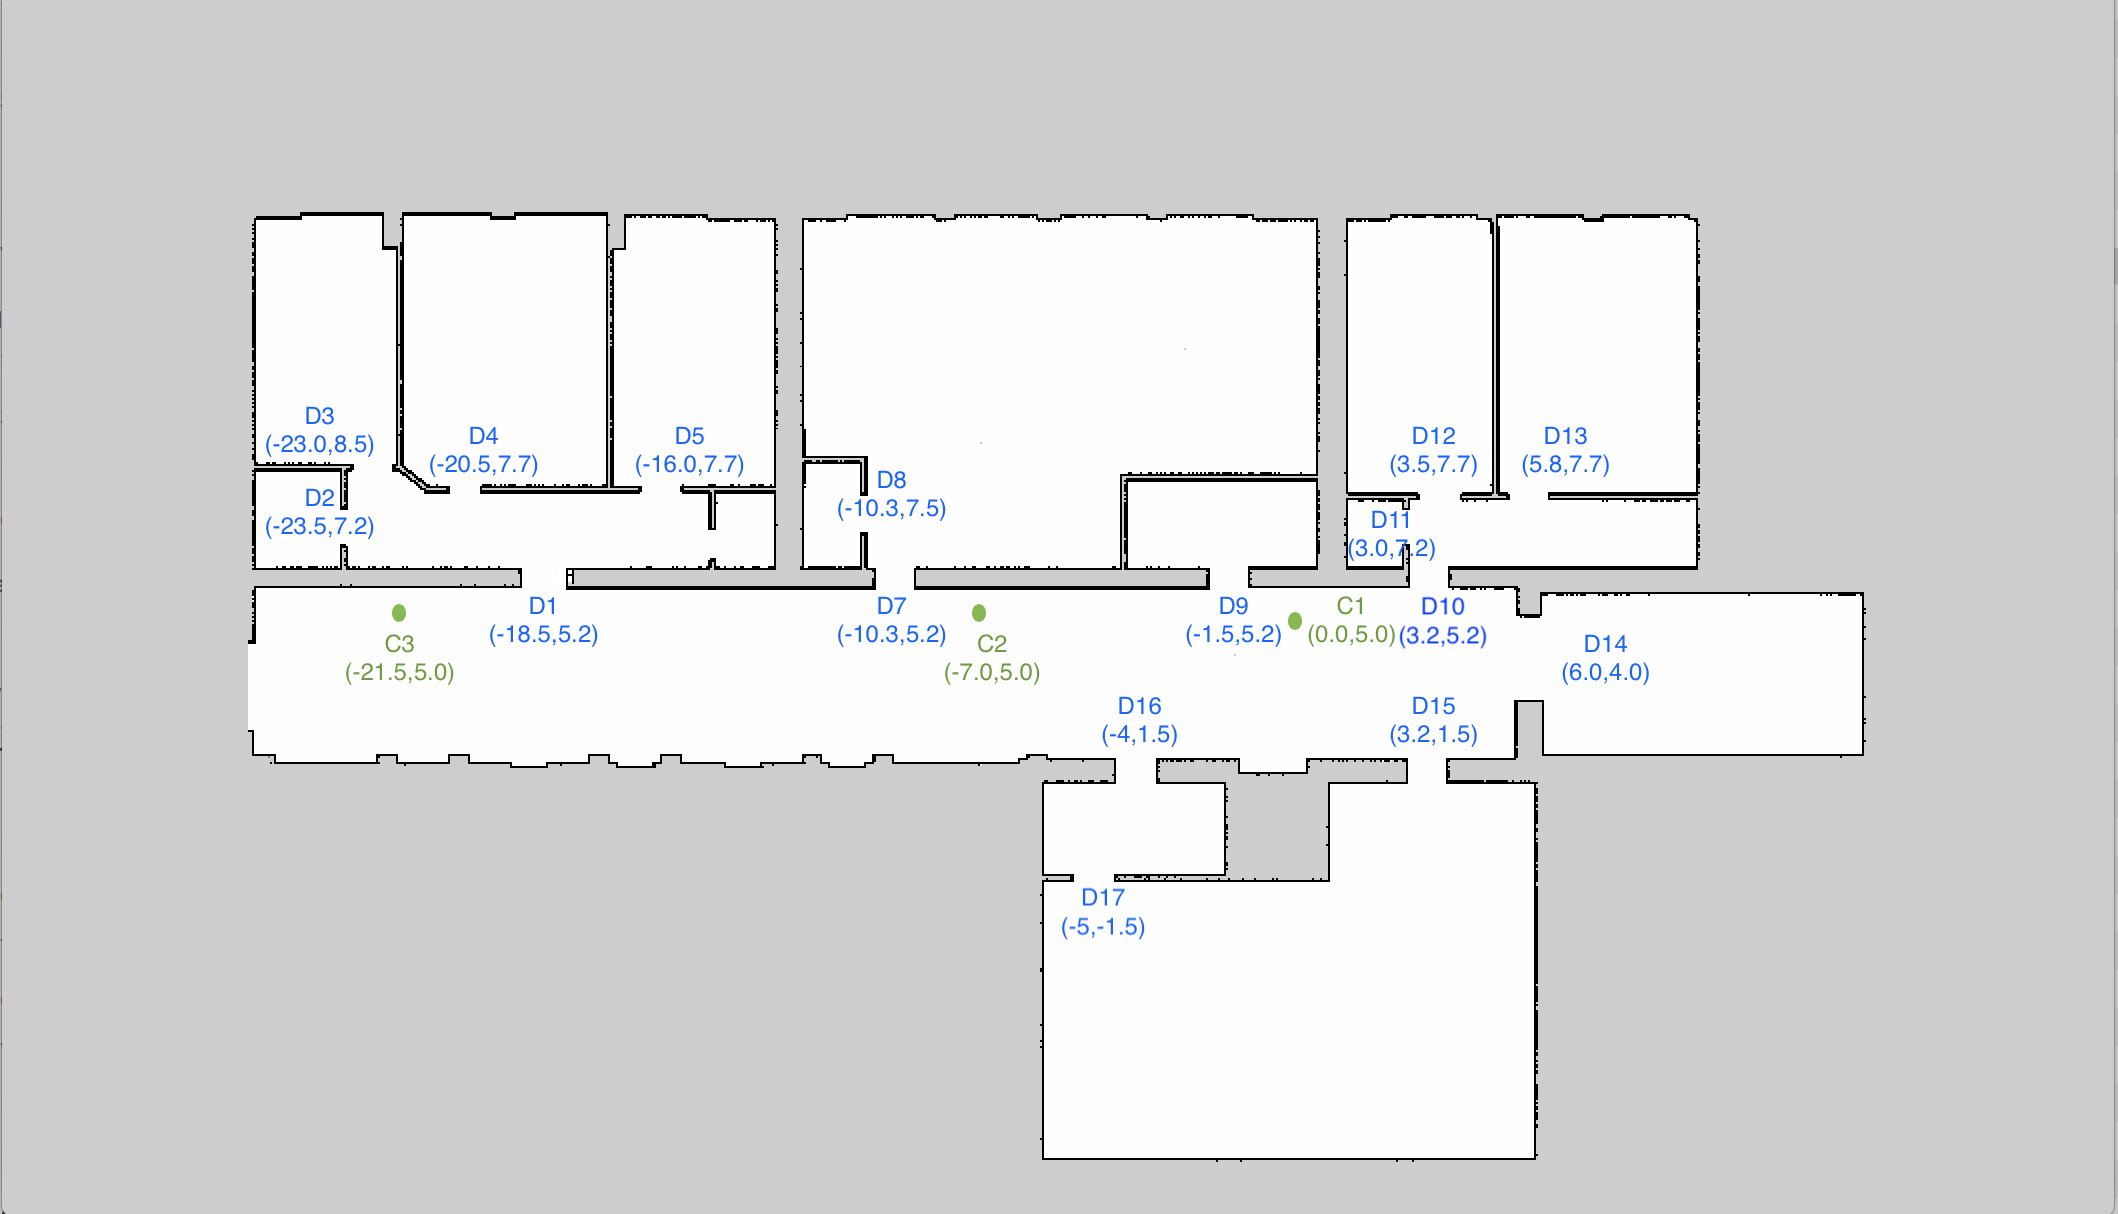
\includegraphics[width = 0.9\textwidth]{content/images/ch3/positions_door_station.png}
	\caption{Positions of Charging Stations (C1-C3) and Doors (D1-D17)}
	\label{fig:positions_door_station}
\end{figure}

\subsection{Gather Environment Infomation Approach}
The goal of this project is to allocate tasks to robots based on the information gathered about room occupancy. However, current robot sensing technology, including robots equipped with external sensors, is not good enough to gather information of whole office enviroment satisfactorily. 
For example, compared with office enviroment, the field within sensing range is rather narrow. Therefore, use of external enviroment information sources is essential to bridge the local knowledge gap.
In this project, since distributed sensor network cost higher than robot and its network connections consume much energy, the fixed sensors capable of short-distance communication are installed in the enviroment. They can share their environment information with robots, thus robots don't need to equip with numerous sensors \cite{PYO2015148}.
Robots interact with sensors while moving in the enviroment and report those enviroment information to centralized pool.
The details about centralized pool storing and studying from enviroment information are discussed in section \ref{sec:task_allocation_procedure}.

%\subsection{Environment Learning}
%IoT system should be adopted in the system enviroment, which can provide enough enviroment information that help multi-robot task allocation system to make decisions. 

%\todo{More Advantages}

\section{Tasks and Task Composition and Decomposition Approach}

\subsection{Task Specification}
Robots should execute tasks in order to achieve the overall system goals: gather information and environmental information continuously for a long time and allocate tasks to robots based on the environmental information.  Therefore, three task names are defined: ``gather enviroment information task'' asks a robot gathers enviroment information from sensors, ``execute task'' asks a robot moves to a point and  ``charging task'' asks robot to refill its battery at charging station.
The task specifications are stored in ``task table'' in database (Table \ref{tab:db_task_table}).


\subsection{Task Composition and Decomposition}
Tasks can be distinguished to ``simple tasks'' and ``Complex tasks''.  ``Simple tasks'' comprises a single action that can be performed by a single robot. A ``Complex tasks'' can be broken up or decomposed into multiple ``small tasks''. Those sub-tasks of a complex task need to be performed by the same robot.
In this project, the centralized poll not only can create ``simple tasks'' according to task specifications (Table \ref{tab:db_task_table}), but also can analyze the dependencies of ``simple tasks'' and form a dependency chain to compose ``complex tasks''. The robot (robot controller) can decompose a ``Complex task'' to ``simple tasks'' and execute ``small tasks'' according to their dependencies.

\section{Multi-robot Task Allocation Approach}
The multi-robot task allocation module in the architecture should perform multi-robot task allocation. 
The implementation of task allocation is shown in Section \ref{sec:task_allocation_procedure}. There are some general rules for multi-robot task allocation.


\begin{enumerate}
	\label{sec:task_allocation_rule}
	\item When the battery of robot belows 10\%, a charging task will be created and allocated to robot.
	\item When the battery of robot aboves 10\%, firstly, ``simple exeucte tasks'' according to the task table in database are created. Secondly, ``complex execute tasks'' will be composed and one of them will be selcted and allocated to robot. To ensure consistency, a ``complex task'' composed by only one ``simple task'' is allowed. 
    \item If there are no ``execute tasks'' in database or after ``execute tasks allocation'', the cost of tasks exceeds the threshold, a ``gather environment task'' will be created and allocated to robot.
\end{enumerate}

\subsection{Execute Task}
As discussed in Section \ref{sec:task_allocation_rule}, one of the ``complex execute tasks'' should be selected for requesting robot. In order to select an ``execute task'', the decision variables and Equation \ref{eq:large_execute_task_cost} are used to calculate the cost. The ``complex execute tasks'' with the lowest cost will be selected.

\begin{equation}
	\label{eq:large_execute_task_cost} 
	\begin{aligned}
	& \mbox{W: Weight } \\
	& \mbox{n: Number of doors} \\
	& \mbox{Cost}_{\mbox{Large execute task}} = \frac{W_{\mbox{battery}} \times \mbox{Battery consumtion}}{n} + W_{\mbox{waiting}} \times \mbox{waiting time} \\
	& + W_{\mbox{possibility}} \times \prod\limits_{i=1}^n \mbox{Door open possibility}  + W_{\mbox{priority}} \times \mbox{Priority}
	\end{aligned}
\end{equation}

\paragraph{Decision variables}
\begin{itemize}
\item \textsl{Task Priority.}  The priority is discussed Section \ref{sec:task_table}.
\item \textsl{Product of Door Open Possibility.} The product of open possibilities of doors on trajectory: All doors that the robot will pass through when moving from its location to the target point.
	An example of ``measurement result'' table is shown in Table \ref{tab:db_measurement_result}, an example of ``open possibility'' table is shown in Table \ref{tab:db_open_possibilities}. 
\item \textsl{Waiting Time. } The waiting time is the difference between the current simulation time and start time of the first task to be executed. $T_{waiting} = T_{first\_task} - T_{now}$
\item \textsl{Battery Consumption.} The Battery Consumption is related to robot trajectory. For a Large ``execute task'' that contains n simple task, Equation \ref{eq:battery_consumption} can be used to calculate battery consumption. The centralized pool will send the task with the lowest cost to this robot.
\end{itemize}


\begin{equation}
\begin{aligned}
\label{eq:battery_consumption}
& \mbox{B:Battery consumption } \\
& \mbox{W: Weight } \\
& \mbox{m: Number of waypoint } \\
& \mbox{n: Number of simple task} \\
& B_{\mbox{complex task}} = \sum_{\mbox{task}_1}^{\mbox{task}_n} B_{\mbox{trajectory}} \\
& = \sum_{t = \mbox{task}_1}^{\mbox{task}_n} \sum_{\mbox{waypoint}_1}^{\mbox{waypoint}_m} [W_{\mbox{position}} \times \mbox{position variation}+W_{\mbox{angle}}  \times \mbox{angle variation}]\\
& = \sum_{t = \mbox{task}_1}^{\mbox{task}_n} \sum_{p = \mbox{waypoint}_1}^{\mbox{waypoint}_m} [ W_{\mbox{position}} \times \sqrt{(x_p-x_{p-1} )^2+(y_p-y_{p-1} )^2} \\
&   + W_{\mbox{angle}} \times 2 \times \arccos(w_p)] 
\end{aligned}
\end{equation}


\subsection{Environment Task}
As is discussed in section \ref{sec:task_allocation_rule}, once there are no suitable tasks in centralized pool, the task allocation module should create a ``gather environment information task'' to gather more measurement results and further more improve the accuracy of ``open possibilities'' table.
To create a ``gather environment information task'', Equation \ref{eq:door_cost} and following decision variables are used to calculate the costs of doors. A ``gather environment information task'' to the door with the lowest cost will be created.

\begin{equation}
	\label{eq:door_cost}
	\begin{aligned}
	& \mbox{W: Weight } \\
	& \mbox{n: Number of doors on trajectory} \\	
	& \mbox{Cost}_{\mbox{door}} = \frac{W_{\mbox{battery}} \times \mbox{Battery consumtion}}{n} + W_{\mbox{time}} \times (T_{\mbox{last update}} - T_{\mbox{now}}) \\
	& + W_{\mbox{possibility}} \times \prod\limits_{i=1}^n \mbox{Door open possibility}
	\end{aligned}
\end{equation}

\paragraph{Decision variables}
\begin{itemize}
	\item \textsl{Door Last Update Time.} The latest timestamp when the door is measured.
	\item \textsl{Product of Door Open Possibility.} The product of open possibilities of doors on trajectory: All doors that the robot will pass through when moving from its location to the front of the target door.
	\item \textsl{Battery Consumption.} The battery consumption is related to the trajectory from robot to the front of the door. Equation \ref{eq:battery_consumption} can be used to calculate battery consumption.
\end{itemize}



\subsection{Charging Task}
As is discussed in section \ref{sec:task_allocation_rule}, once a robot sends task request to the centralized pool, the centralized pool should figure out whether this robot need charging, if yes it should create a ``charging task'' for requesting robot. 
To create a ``charging task'', Equation \ref{eq:door_cost} and following decision variables are used to calculate the costs of charging station. A ``charging task'' to the charging station with the lowest cost will be created.

\begin{equation}	
\label{eq:charging_station_cost}
\begin{aligned}
	& \mbox{W: Weight } \\
	& \mbox{Cost}_{\mbox{charging station}} = \frac{W_{\mbox{battery}} \times \mbox{battery consumtion}}{n} + W_{\mbox{time}} \times T_{\mbox{remain}}
\end{aligned}
\end{equation}


\paragraph{Decision variables}
\begin{itemize}
	\item \textsl{Remain Time.} It describes how long will a charging station be free. 
	\item \textsl{Battery Consumption.} Similar to ``execute task'' allocation, the battery consumption is related to the trajectory from robot to the charging station. Equation \ref{eq:battery_consumption} can be used to calculate battery consumption.
\end{itemize}

	%Approach
\chapter{Implementation}

%Explain what you did to implement your solution, problems that occurred and how you fixed them. 
%If they are interesting, include some relevant parts of the implementation (most relevant pieces of code and so on). 

\section{Communication Protocols}


Centralized pool and robots need to share task information with each other. There are some basic requirements for communication: firstly,
robot should initiate the communication once it has finished all task in task queue and get free. This is solved by assigning robot controller as ROS service client and centralized pool as ROS service server.
This method saves unnecessary communication cost by avoiding keep tracking the current position, availability and states of all robots.
Secondly, robot should forward sensor data to centralized pool while processing a task. This is solved by assigning robot controller as ROS action server and centralized pool as ROS action client.
As is shown in \ref{fig:comminication}, an efficient communication protocols is designed. 

\subsection{Message about Measurement}
\label{sec:measurement_message}
When a robot pass by a door, it will receive messages from sensor. 
In order to save resources, instead of a system enviroment in real life, a door simulator ROS node is used to publish all measurement result for all doors. The message formart is shown in Table \ref{tab:sensor_message} 
The measurement results(opened and closed) are created according to the "open possible" column in the "open possibilities" table (Figure \ref{fig:database_er}).

\begin{table}[htb]
\centering
\begin{tabular}{|c|c|c|c|c|} 
\hline
Door ID  & Position& Timestamp & Measurement Result \\
\hline\hline
1&(-18.5,5.2) & 2020-06-01 9:00:02 & Door opened \\ [1ex] 
\hline
\end{tabular}
\caption{Measurement Message Format and Example}
\label{tab:sensor_message}
\end{table}
	

\subsection{Message about Task}
\label{sec:task_message}
Four types of message are defined: 
(1)Task request message(Table\ref{tab:request_message}); (2) Task goal messages(Table \ref{tab:goal_message}); (3) Task feedback message (Table \ref{tab:feedback_message}); (4) Task result message (Table \ref{tab:result_message}). 

\begin{figure}[htbp]
    \centering
    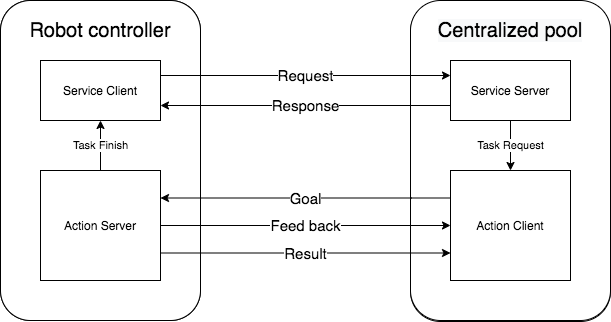
\includegraphics[width = 0.7\textwidth]{content/images/ch4/robot_pool_comminication.drawio.png}
    \caption{Communication between Robot and Centralized Pool}
    \label{fig:comminication}
\end{figure}

\begin{table}[htb]
\centering
\begin{tabular}{|c|c|c|} 
\hline
Battery & Pose & Robot ID\\
\hline\hline
93	&(2,4)	&1 \\ [1ex] 
\hline
\end{tabular}
\caption{Request Message Format and Example}
\label{tab:request_message}
\end{table}

\begin{table}[htb]
\centering
\resizebox{\textwidth}{!}{
\begin{tabular}{|c|c|c|c|} 
\hline
Task id[] &Task type & Target id & Goal[] \\
\hline\hline
1& Gather Environment Info & 9	& (-1.5,5.2) 2020-06-01 9:00:00 \\
\hline
[3,4]	& Execute task & 21, 22	& (-24.0,12.0), 2020-06-01 9:02:00 (-21.0,12.0) 2020-06-01 9:02:00 \\
\hline
5	& Charging	& 17	&(0.0,5.0), 2020-06-01 9:04:00 \\ [1ex] 
\hline
\end{tabular}}
\caption{Action Goal Message Format and Example}
\label{tab:goal_message}
\end{table}

\begin{table}[htb]
\centering
\begin{tabular}{|c|c|c|c|} 
\hline
Robot id & Door id & Measurement time & Measurement result \\
\hline\hline
1	& 3	& 2020-06-01 9:00:03 & Door open \\ [1ex] 
\hline
\end{tabular}
\caption{Action Feedback Message Format and Example}
\label{tab:feedback_message}
\end{table}

\begin{table}[htb]
\centering
\begin{tabular}{|c|c|c|} 
\hline
Task id	& Task type	& Result\\
\hline\hline
1 & Gather Enviroment Info & Success \\ [1ex] 
\hline
\end{tabular}
\caption{Action Result Message Format and Example}
\label{tab:result_message}
\end{table}


\begin{figure}[htbp]
    \centering
    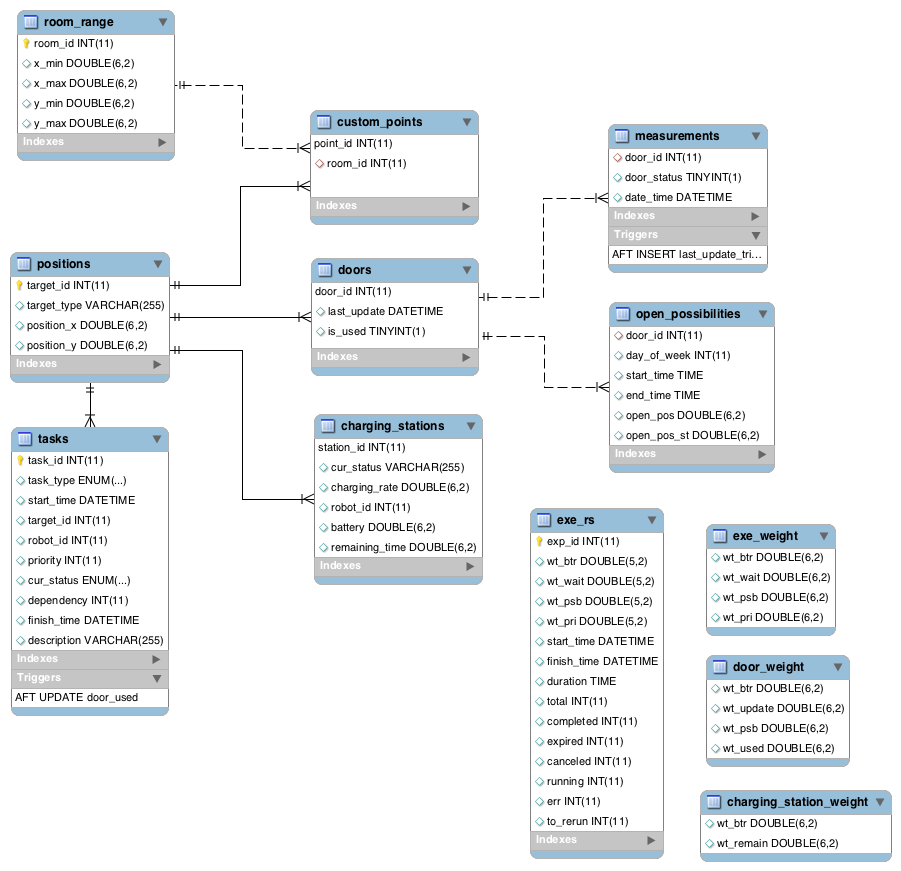
\includegraphics[width = 0.7\textwidth]{content/images/ch4/database_er.png}
    \caption{Database Entity Relationship Diagram}
    \label{fig:database_er}
\end{figure}


\section{Database}
The centralized pool keep information it requires, to make decisions. Figure \ref{fig:database_er} shows the relationship between entities. Following are explanations of some tables.
\begin{itemize}
	\item \textsl{Table doors.} Table doors stores enviroment information. In table doors, the is\_used column will be updated when an Enviroment-task to this door is updated. The last update will be updated when the centralized pool receive a new measurement result. 
	\item \textsl{Table open\_ossibilities.} Table open\_ossibilities is based on the statistic of door measurement in a specific time period of each working day. These two table will be updated when centralized pool receive a new measurement result. 
	\item \textsl{Table exe\_rs.} Table exe\_rs stores experiment result while table exe\_weight, table door\_weight and table charging\_station\_weight stores weight values for experiment. Chapter 5 introduces the details of experiment.
	\item \textsl{Table costum\_points.} When user gives the system a task, the target point of this task will be stored in position table, and a target\_id will be generated.  This target\_id will be stored in custum\_point table. 	Additionally, with the information in room\_range table, the system will recognize which room does the point belong to and write room\_id column in costom\_points table.
\end{itemize}


\section{Procedure}
As stated in the Chapter 3, the goal of task scheduling is finishing all tasks as soon as possible while keep the cost as low as possible. 
The task assignment and execution happends at two level. \cite{Ivan2017} the task and the path planner solves a planning problem. It takes and occupancy grid, a specific robot and a set of task specifications, and generates trajectorys for each task. According to those trajectorys and task specifications, the task with the lowest cost is assigned to robot.
At the dynamic level, after each robot receive a task, it runs a navigation stack to execute this task stepwise. Each robot computes a local trajectory but takes into account dynamic obstacles.
The process of the robot task allocation system is as follows.


\begin{figure}[htbp]
    \centering
    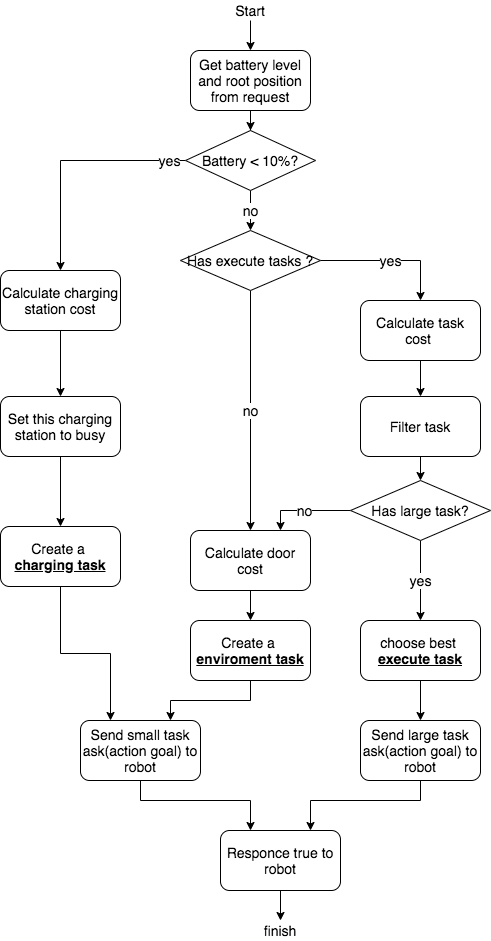
\includegraphics[width = 0.7\textwidth]{content/images/ch4/centralized_task_select.drawio.png}
    \caption{Centralized Pool Task allocation}
    \label{fig:centralized_task_allocation}
\end{figure}
\subsection{Centralized Pool}

\paragraph{Task Allocation}
When the centralized pool receives a task request (Table \ref{tab:request_message}) from robot, it performs task allocation. The task allocation algorithm is discussed in Section \ref{sec:task_allocation}. The process of task allocation is shown in Figure \ref{fig:centralized_task_allocation}. 
\begin{enumerate}
	\item When the battery of robot belows 10\%, the centralized pool create a charging task to the charging staion with the lowest cost.
	\item When the battery of robot aboves 10\%, the centralized pool loads execute-tasks in database, then combine small tasks with dependencies into large tasks, finally calculates task costs and select one large task with the lowest cost. 
	\item If there are no suitable tasks, a gather-enviroment-task to the door with the lowest cost is generated. 
\end{enumerate}
The difference between task is discussed in Section \ref{sec:task_specifications}. The output of the task allocation includes: task ID, goal coodinate, timestamp and selected robot ID. The task is sent to the selected robot, and the robot performs the tasks.

\paragraph{Handle Task Feedback.}
When the centralized pool receives a task feedback (Table \ref{tab:feedback_message}) that contains a new measurement result from robot, it will add a record in measurement table and update "open possibilities" table in database.

\paragraph{Handle Task Result.}
When the centralized pool receives a task result (Table \ref{tab:result_message}), it updates "tasks" table (Figure \ref{fig:database_er}). The failed "execute tasks" will be reused while the failed others will be marked as "Cancel" or "Error"(Figure \ref{fig:centralized_task_handle}).

\begin{figure}[htbp]
    \centering
    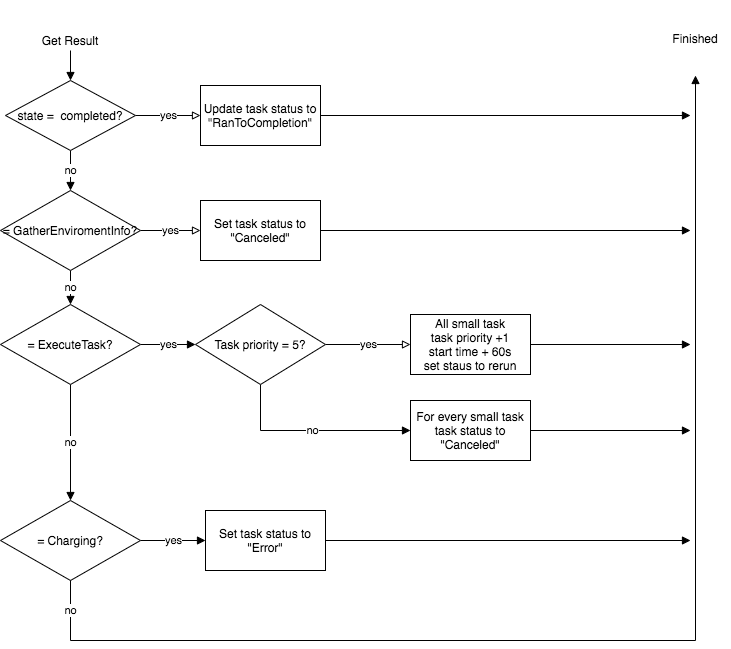
\includegraphics[width = 0.7\textwidth]{content/images/ch4/centralized_task_result.drawio.png}
    \caption{Centralized Pool Handle Task Result}
    \label{fig:centralized_task_handle}
\end{figure}


\subsection{Robot}

\begin{figure}[htbp]
    \centering
    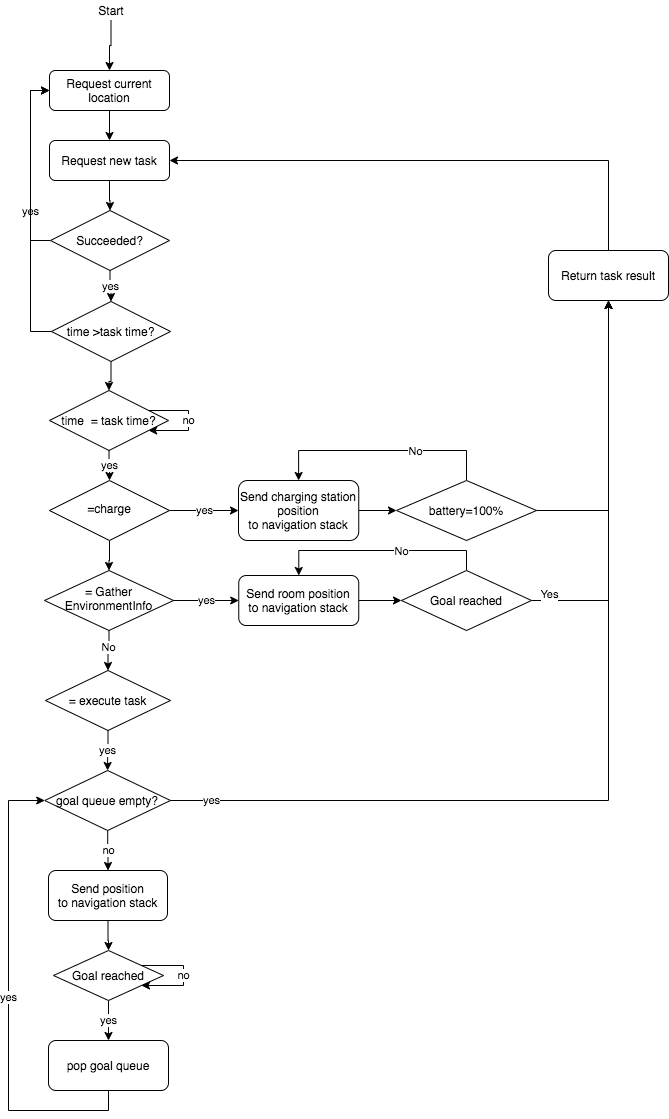
\includegraphics[width = 0.7\textwidth]{content/images/ch4/robot_process_task.drawio.png}
    \caption{Robot Process Task }
    \label{fig:task_process_robot}
\end{figure}

\paragraph{Robot Process Tasks}
When the task queue(Figure \ref{fig:system_architecture}) in a robot is empty, robot requests a new task. If the robot gets a "charging task", it will move to the position of charging staion(Figure \ref{fig:positions_door_station}) and interact with charging station node (Section \ref{sec:charging_station}).
When a robot gets an "execute task" which is a large task, it will move to all goals in order.
When a robot gets a "gather enviroment information" task, it will move to the door's position.
During task processing, the timer checks periodically the status of navigation stack. If any errors occurs, the robot send a "failed" result with description to the centralized pool.  
When task compltes without error, the robot will send "Succedded" result to the centralized pool.


\begin{figure}[htbp]
    \centering
    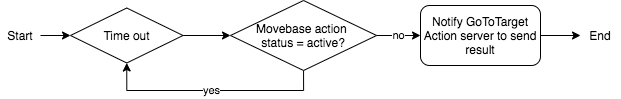
\includegraphics[width = 0.7\textwidth]{content/images/ch4/robot_timer.drawio.png}
    \caption{Robot Timer}
    \label{fig:robot_timer}
\end{figure}

\begin{figure}[htbp]
    \centering
    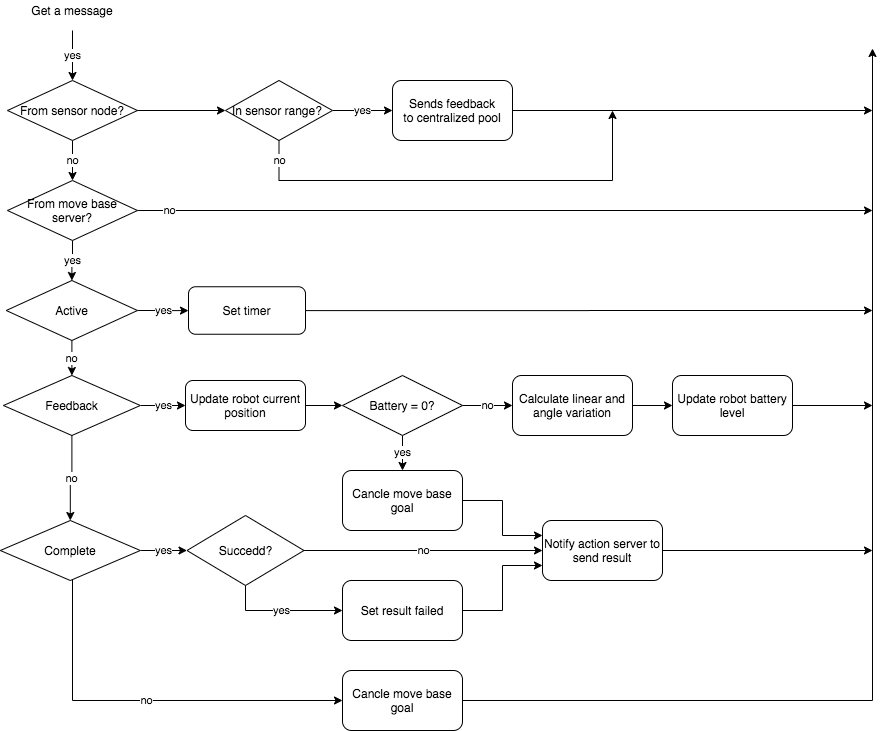
\includegraphics[width = 0.7\textwidth]{content/images/ch4/robot_message.drawio.png}
    \caption{Robot Hanlde Message}
    \label{fig:robot_handle_message}
\end{figure}

\paragraph{Robot Handle Messages}
While a robot is processing a task, it listens to door sensors and forwards measurement result to the centralized pool. 
Besides sensor messages, it receives messages from move\_base node. The details of robot message handling is shown in Figure \ref{fig:robot_handle_message}.

\subsection{Charging Station}
\label{sec:charging_station}
The charging station consist of a charging station node and "charging station" table in database (Table \ref{fig:database_er}). 
When a robot arrives the position of charging staion, it will start interacting with charging station node. Firstly it sends battery level and its robot ID to charging station. 

\begin{figure}[htbp]
    \centering
    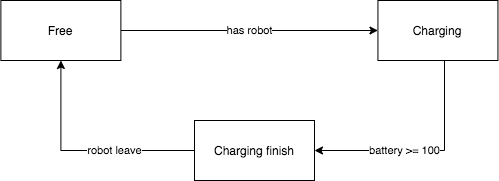
\includegraphics[width = 0.7\textwidth]{content/images/ch4/charging_station_state_machine.drawio.png}
    \caption{Charging Station State Machine}
    \label{fig:charging_station_state_machine}
\end{figure}

\begin{figure}[htbp]
    \centering
    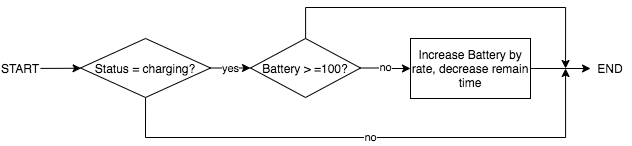
\includegraphics[width = 0.7\textwidth]{content/images/ch4/charging_station_charging_event.drawio.png}
    \caption{Charging Station Scheduled Charging Event}
    \label{fig:charging_station_event}
\end{figure}

\begin{figure}[htbp]
    \centering
    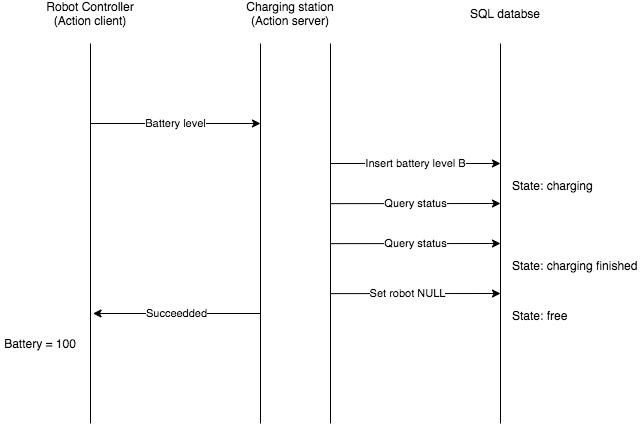
\includegraphics[width = 0.7\textwidth]{content/images/ch4/charging_station_message.drawio.png}
    \caption{Charging Station Message}
    \label{fig:charging_station_message}
\end{figure} %Implementation
\chapter{Evaluation}


%In this chapter you should describe the previous (if possible) and final experiments performed on the implementation.

%Every single experiment should be explained individually, providing to the reader information about the meaning of the experiment, the expected (theoretical) results, the final results, the comparison between them and others (if possible) and the conclusions. 

%Each experiment should include a description, covering (when possible) the following information:
%\begin{itemize}
%	\item Significant physical features (obstacles present on the environment, human presence, temperature, humidity, possible noise sources, computational speed of the machine, etc.)
%	\item The precise location of the experiment (latitude and longitude, room number or citation to a description of the used laboratory).
%	\item Sampling design (variable(s) measured, transformation performed to the data, samples collected, replication, comparative with a Ground Truth system, collecting data protocol).
%	\item Analysis design (how the data are processed, statistical procedures used, statistical level to determine significance).
%\end{itemize}
%The provided information should be sufficient to allow other scientists to repeat your experiment in the same conditions. Thus, the use of standard and well-known equipment could only be represented by a simple sentence, but the non-standard equipment should be described in detail, citing the source (vendor) and most important characteristics.

%To write it, try to use the third person when describing the experiments and results. Avoid to use first person. Past tense should be the dominant conjugation (the work is done and was performed in the past).

%Note: Graphics represent really well data, use them! (Matlab or Octave could be useful for that).
Simulation experiment were conducted using a multirobot simulation enviroment(Figure \ref{fig:gazebo_model}) Gazebo. As discussed in section \ref{sec:system_enviroment}, the map (Figure \ref{fig:exp_map}) is greated by SLAM \cite{slam}. The are important coordinates: D1-D17 represent doors; C1-C3 represent charging stations; P1-P10 represent points used as goal positions in experiments.
Followings are goals of experiments:

\begin{itemize}
	\item Evaluate the need of decition variables.
	\item Find the best weight combinations in cost functions.
%	\item Investigate how different weight combinations in cost functions affact the performance \cite{Shiqi}. 
\end{itemize}

\begin{figure}[htbp]
	\centering
	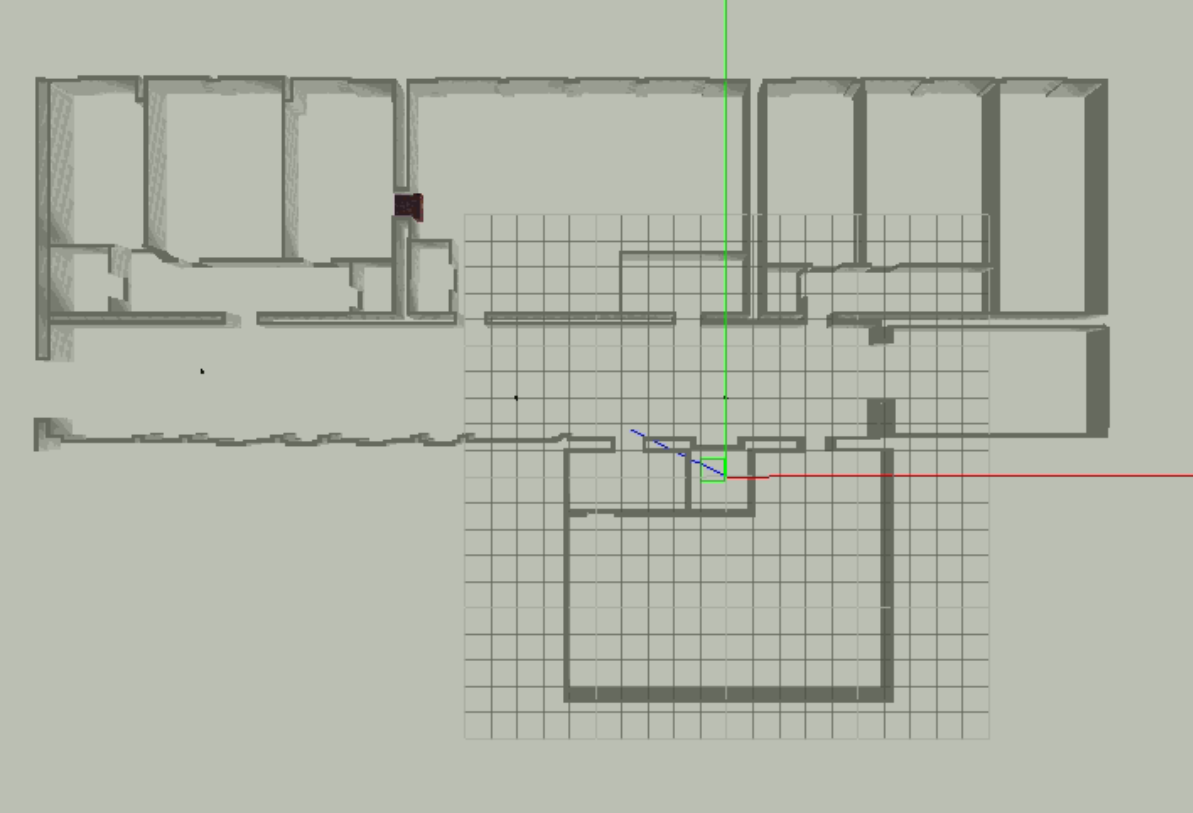
\includegraphics[width = 0.7\textwidth]{content/images/ch5/gazebo_model.png}
	\caption{Gazebo Simulation}
	\label{fig:gazebo_model}
\end{figure}

\begin{figure}[htbp]
    \centering
    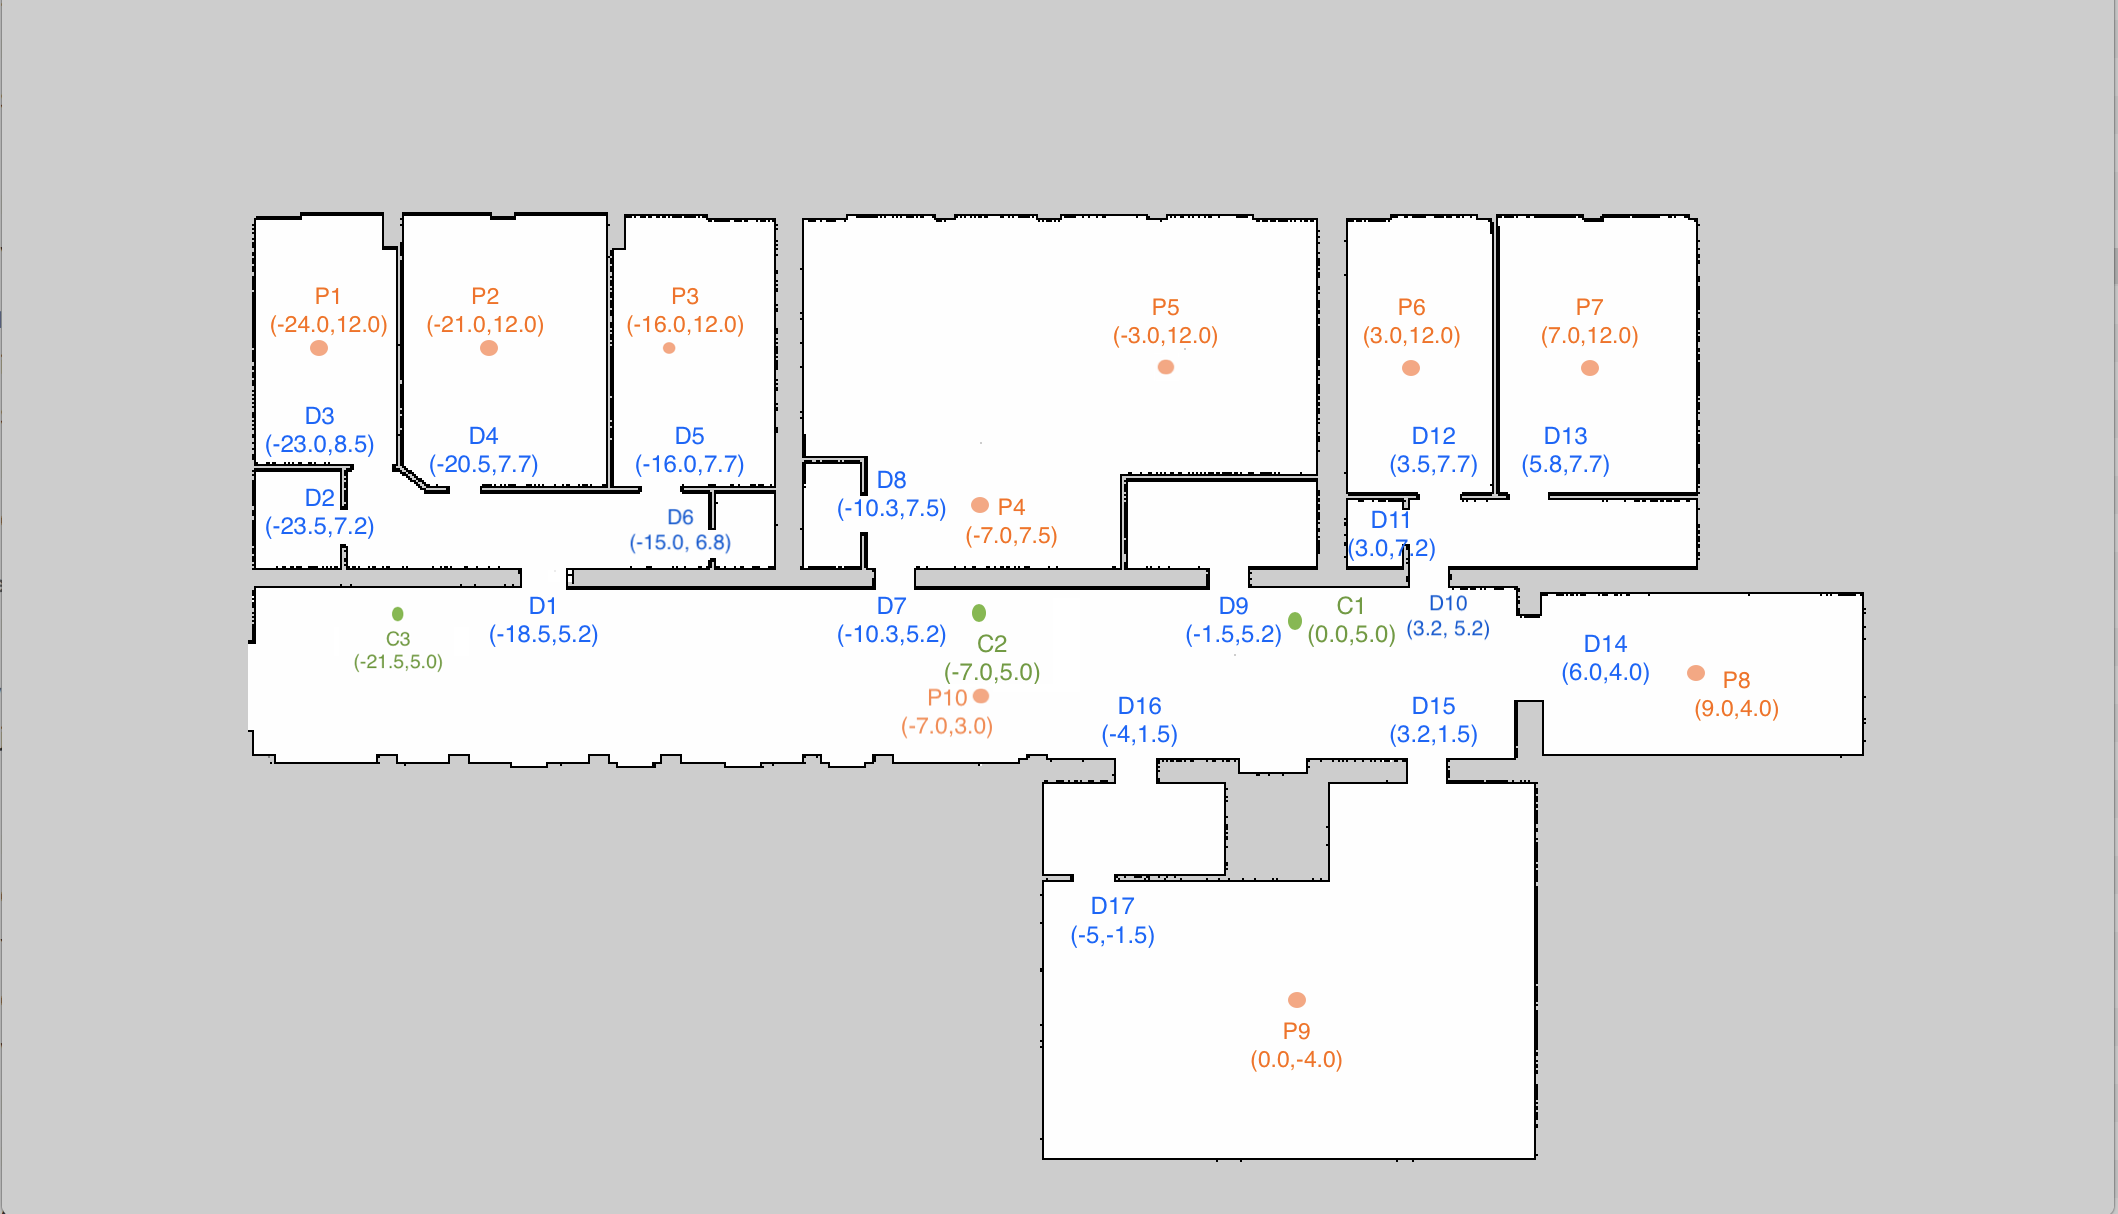
\includegraphics[width = 0.9\textwidth]{content/images/ch5/door_station_points.png}
    \caption{Experiment Map}
    \label{fig:exp_map}
\end{figure}

\section{Execute Task Evaluation}

\paragraph{Experiment precondition}
There are some preconditions for every experiment. When simulation started, robots moved to corresponding charging station and started charging. For example, robot 1 charged at charging staion 1, robot 2 charged at charging staion 2, robot 3 charged at charging staion 3(Figure \ref{fig:execute_task_experiment_timeline}). 
Once robot fully charged, the next experiment started, and 15 execute tasks are created. Especially, for each experiment, tasks with the same ID has the same start time and the same goal position. When all robot finished tasks, the experiment finished.
These rules ensure that robot would not only start at same initial points but also process same task and not shut down because of power exhaustion.

\begin{figure}[htbp]
    \centering
    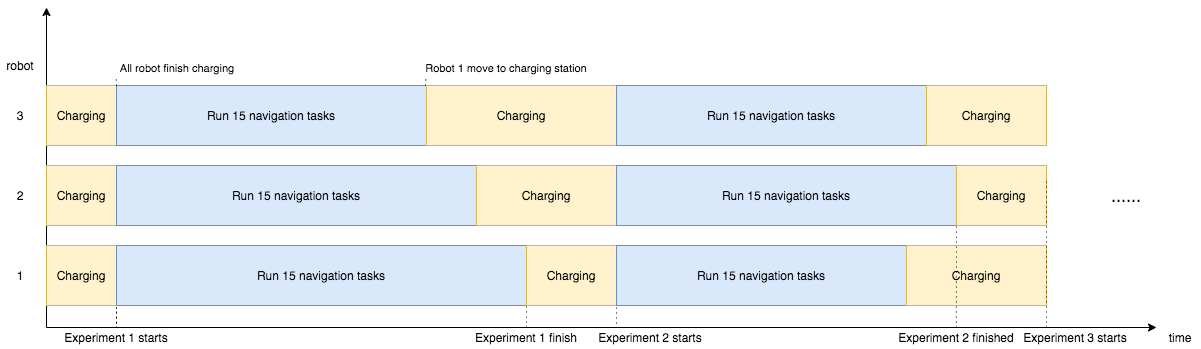
\includegraphics[width = 0.9\textwidth]{content/images/ch5/exe_exp_timeline.drawio.png}
    \caption{Execute Task Experiment Timeline}
    \label{fig:execute_task_experiment_timeline}
\end{figure}

\subsection{Experiment: Need of decision variables}
As discussed in Section \ref{sec:exe_task_allocation}, there are four decision variables: battery consumption, waiting time, product of door open possibility and priority. 
The first set of experiments evaluated the need of decition variables in cost function. 
The experiment result (Table \ref{tab:exp_decision_variables}) shows that the experiment 1 used the minimum time and all 15 task are completed.
The experiment with decision variables cost function with multiple decision variables has better performance than a cost function with single decition variable.

\begin{table}[htb]
\centering
\resizebox{\textwidth}{!}{
\begin{tabular}{|c|c|c|c|c|c|c|c|c|c|c|c|} 
\hline
&\multicolumn{4}{|c|}{Weight Combination} & \multirow{2}{*}{Experiment Duration}& \multicolumn{3}{|c|}{Task Statistic}\\
\cline{1-5}\cline{7-9}
Experiment ID	& 	 Battery Consumption & Waiting Time & Door Open Possibility	&  Priority & ~	& Total	 & Completed &	 Expired	 \\
\hline
1	& 1.00 &	 1.00 &	 -1.00&  -1.00&	 00:18:23 &	 15 &	 15 &	 0	 \\
\hline
2	& 1.00 &	 0.00 &	 0.00 &	 0.00 &	 00:17:23 &	 15 &	 7 &	 8	\\ 
\hline
3	& 0.00 &	 1.00 &	 0.00 &	 0.00 &	 00:18:56 &	 15 &	 15 &	 0	 \\
\hline
4	& 0.00 &	 0.00 &	 -1.00 & 0.00 &	 00:18:41 &	 15 &	 5 &	 10	\\
\hline	 
5	& 0.00 &	 0.00 &	 0.00 &	 -1.00&	 00:17:21 &	 15 &	  3 &	 12	 \\	 
\hline
\end{tabular}}
\caption{Runing execute task with single decision variable and multiple decision variables}
\label{tab:exp_decision_variables}
\end{table}

\subsection{Experiment: Find the best weight combinations}

The 


 %Evaluation
\chapter{Discussion}

The meaning of this paragraph is to interpret the results of the performed work. It will always connect the introduction, the postulated hypothesis and the results of the thesis/bachelor/master.

It should answer the following questions:
\begin{itemize}
	\item Could your results answer your initial questions?
	\item Did your results agree with your initial hypothesis?
	\item Did you close your problem, or there are still things to be solved? If yes, what will you do to solve them? 
\end{itemize}
	%Discussion
\chapter{Acknowledgements}

% (This part is optional, and it could be completely excluded by deleting \\ 
% \textbf{ \textbackslash include \{content/chapters/chapter7\}} \\
% from the Firstname\_Lastname\_Diplom\_Master\_arbeit.tex file)

% This paragraph could mention people or institutions that supported you to some extent with your work or friends and relatives that supported you during your study period. 

I would like to begin by thanking my supervisor Dr. Matteo Zella and Carlos Medina Sanchez. Their strict attitude and enthusiasm for research have encouraged me. Many thanks for their reading and examining my thesis. I can not finish my thesis without their guidance.

I also would like to thank all the people who have supported me during writing. I am so lucky to study at the University Duisburg-Essen.	%Aknowledgments


% Appendix chapters to be put here. They will be enumerated with capital letters
% if you  did not change the \documentclass options.
\begin{appendix}


%\include{appendix_chapterA}
\end{appendix}
%Ende Anhang

%Bibliography
% We strongly recommend to use bibtex to manage your bibliography. It helps you
% structure your references and helps avoiding missing important data for a correct
% quotation. If you have no other idea jabref (http://jabref.sourceforge.net/)
% might be a good idea (Jave runtime environment needed).
% This style is good to use in german master thesis'. You need to have activated
% \usepackage{bigerm} above.
% For english documents just use apalike.
\bibliographystyle{geralpha}


% to finally announce where your bibliography is stored use
\bibliography{content/references/references}
% it is also possible to have several files separated by comma.
%Bibliographie Angaben mit \bibliography{}

%pagenumbering{null}

\ 

%clearpage
\cleardoublepage

\ 


\pagestyle{empty}
\vfill
\textbf{Versicherung an Eides Statt}\\

\[German\] Hiermit versichere ich, dass ich die vorliegende Bachelor(Master)arbeit selbst�ndig - mit Ausnahme der Anleitung durch die Betreuer - verfasst, keine anderen als die angegebenen Quellen und Hilfsmittel benutzt, sowie Zitate kenntlich gemacht habe. Ich versichere dass ich alle entsprechenden Angaben nach bestem Wissen und Gewissen vorgenommen habe, dass sie der Wahrheit entspechen und dass ich nichts verschwiegen habe. Mir ist bekannt, dass eine falsche Versicherung an Eides Statt nach \S 156 und nach \S 163 Abs. 1 des Strafgesetzbuches mit Freiheitsstrafe oder Geldstrafe bestraft wird.\\

\[English\] I hereby declare that I have written this Bachelor (Master) thesis - except for the guidance of the supervisor - independently, using no other than the specified sources and resources, and that all quotations have been indicated. I declare that I have reported to the best of my knowledge all the relevant information, that it is true and that I concealed nothing. I am aware that a false declaration will be punished according to \S 156 and \S 163 par. 1 of the criminal code with a prison sentence or a monetary penalty.\\
\\\\
Essen, \today\\
$\overline{\parbox{4cm}{(Ort, Datum)}} ~~~~~~~~~~~~~~~~~~~~~~~~~~~ \overline{\parbox{5cm}{\studentFirsName { } \studentSecondName}}$
 %It may be necessary that you replace "Bachelorarbeit" with "Masterarbeit" here...

\end{document}
%%% Local Variables:
%%% mode: latex
%%% TeX-master: t
%%% End:
